% ===========================================================================
% BRCA Multi-Omics Data Mining — LaTeX Academic Paper
% Compile: xelatex -> bibtex -> xelatex -> xelatex
% ===========================================================================
\documentclass[12pt,a4paper]{ctexart}

% ---------- Packages ----------
\usepackage[top=2.5cm, bottom=2.5cm, left=3cm, right=2.5cm]{geometry}
\usepackage{graphicx}
\usepackage{booktabs}
\usepackage[labelfont=bf,font=small]{caption}
\usepackage{subcaption}
\usepackage[hidelinks]{hyperref}
\usepackage{amsmath}
\usepackage{float}
\usepackage{array}
\usepackage{longtable}

% ---------- Bibliography: GB/T 7714-2015 ----------
\usepackage[backend=biber,style=gb7714-2015]{biblatex}
\addbibresource{references.bib}

% ---------- Figure path ----------
\graphicspath{{../results/figures_pub/}}

% ---------- Title ----------
\title{\heiti\zihao{3} 基于多组学数据挖掘的乳腺癌分子特征分析}
\author{}
\date{}

\begin{document}

\maketitle

% ==================== 摘要 ====================
\begin{abstract}
\noindent
乳腺癌是全球发病率最高的恶性肿瘤，其分子异质性是精准诊疗面临的核心挑战。本研究基于TCGA-BRCA多组学数据（mRNA转录组25,981个基因、miRNA表达谱1,881个、体细胞突变15,413个基因及临床注释94项），对1,076例多组学共同患者进行了系统性的数据挖掘分析。研究综合运用DESeq2差异表达分析、LASSO多分类回归、随机森林分类、加权基因共表达网络分析（WGCNA）、Cox比例风险回归、maftools突变景观分析、g:Profiler功能富集分析、arules关联规则挖掘及ConsensusClusterPlus共识聚类等算法，构建了从数据预处理到生物学发现的全流程分析管线。主要结果包括：鉴定6,768个显著差异表达基因（$|\log_2\text{FC}|>1$, FDR$<0.05$），其中上调4,334个、下调2,434个；LASSO分类器以89.4\%准确率实现三分类分子亚型预测；WGCNA识别9个共表达模块，blue模块枢纽基因模块隶属度达0.959；多变量Cox模型C-index为0.771，Stage IV风险比达8.74；PIK3CA（37.3\%）和TP53（35.2\%）为最高频突变基因。功能富集分析揭示上调基因显著富集于细胞周期通路。本研究为乳腺癌多组学数据挖掘提供了完整的分析框架和可复现的计算流程。

\vspace{1em}
\noindent\textbf{关键词}：乳腺癌；TCGA；多组学数据挖掘；差异表达分析；WGCNA；预后模型；功能富集
\end{abstract}

\newpage

% ==================== 1 引言 ====================
\section{引言}

\subsection{研究背景}

据国际癌症研究机构（IARC）GLOBOCAN 2022统计，全球每年新发癌症约2,000万例，死亡约970万例。其中女性乳腺癌以约230万例新发病例居全球恶性肿瘤发病率首位，同年导致约67万例死亡\cite{sung2024global}。乳腺癌的发生发展涉及多基因突变累积、表观遗传重塑及信号通路交互失调等复杂的分子过程\cite{hanahan2011hallmarks}。高通量测序技术的快速发展使大规模、多层次癌症基因组数据的积累成为可能。以癌症基因组图谱（The Cancer Genome Atlas, TCGA）为代表的国际大型合作项目，为研究者提供了涵盖基因组、转录组、表观基因组及蛋白质组的海量公开数据资源\cite{tcga2012comprehensive}。将差异表达筛选、网络建模、正则化回归、聚类分析及关联规则挖掘等数据挖掘方法系统应用于乳腺癌多组学数据的整合分析，不仅有助于识别新的分子标志物和预后预测因子，也可为药物靶点发现和个体化治疗方案的制定提供数据驱动的视角。

\subsection{乳腺癌分子分型}

乳腺癌是由多种分子特征各异的亚型构成的异质性疾病集合。Perou等\cite{perou2000molecular}于2000年首次基于基因表达谱提出乳腺癌分子分型体系，目前国际广泛认可的固有分子亚型（Intrinsic Subtypes）包括四类：（1）Luminal A型，约50\%--60\%，ER+/PR+/HER2-/Ki-67低表达，预后最佳；（2）Luminal B型，约15\%--20\%，ER+但Ki-67较高，HER2可阳性或阴性；（3）HER2过表达型（HER2-enriched），约10\%--15\%，以ERBB2基因扩增为驱动特征；（4）三阴性型（Triple Negative/Basal-like），约15\%--20\%，ER-/PR-/HER2-，侵袭性最强。尽管四分类体系已广泛应用于临床实践，同一亚型内部的生物学异质性仍然显著，整合多组学数据进一步挖掘分子分型的内在结构具有重要的研究价值。

\subsection{数据挖掘在癌症研究中的应用}

在差异表达分析方面，基于负二项分布的DESeq2\cite{love2014moderated}和基于经验贝叶斯的limma是应用最广泛的两套框架。在网络分析层面，加权基因共表达网络分析（WGCNA）\cite{langfelder2008wgcna}通过构建无标度拓扑网络将海量基因聚类为共表达模块。在预后模型构建方面，LASSO-Cox比例风险模型\cite{simon2011regularization}能有效应对高维表达数据中的维数灾难问题。在功能富集方面，g:Profiler\cite{kolberg2023gprofiler}等在线工具提供了一站式多数据库富集分析。在关联模式发现方面，Apriori算法\cite{agrawal1994fast}可从离散化表达数据中挖掘基因与临床特征之间的频繁共现模式。在分子分型方面，共识聚类\cite{wilkerson2010consensus}通过重采样评估聚类稳定性。

\subsection{研究内容与组织结构}

本研究以TCGA-BRCA乳腺癌多组学数据为研究对象，综合运用多种数据挖掘方法，系统开展乳腺癌分子特征的整合分析。论文组织结构如下：第2章介绍数据来源与预处理流程；第3章系统阐述各项数据挖掘算法及分析结果；第4章展示多维度可视化分析；最后为结论与展望。

% ==================== 2 数据来源与预处理 ====================
\section{数据来源与预处理}

\subsection{TCGA-BRCA数据概述}

TCGA由美国NCI和NHGRI于2006年联合启动，覆盖33种癌症类型、超过20,000例肿瘤样本\cite{tcga2012comprehensive}。乳腺浸润性癌（BRCA）是TCGA最早启动的癌种之一，也是样本量最大的实体瘤项目。本研究从Genomic Data Commons（GDC）获取Level 3处理级别的数据，涵盖四个核心数据层：mRNA转录组（HiSeq RNA-seq, STAR-Counts流程）、miRNA转录组（HiSeq miRNA-seq, BCGSC miRNA Profiling）、体细胞突变（WES, MuTect2变异检测流程）及临床信息（TCGA Clinical模块）。TCGA样本条形码前12个字符构成患者级唯一标识符，是多组学数据集成的核心锚点。

\begin{table}[htbp]
\centering
\caption{多组学数据集总览}
\label{tab:data_overview}
\begin{tabular}{lllll}
\toprule
数据层 & 测序平台 & 特征数 & 样本量 & 归一化 \\
\midrule
mRNA表达 & HiSeq RNA-seq & 25,981个基因 & 1,094（肿瘤）+ 113（正常） & TPM \\
miRNA表达 & HiSeq miRNA-seq & 1,881个miRNA & 1,079例 & — \\
体细胞突变 & WES (MuTect2) & 15,413个基因 & 990例 & — \\
临床数据 & TCGA Clinical & 25个核心变量 & 1,174例 & — \\
\bottomrule
\end{tabular}
\end{table}

\subsection{数据获取与整合}

所有多组学数据通过TCGAbiolinks R包\cite{colaprico2016tcgabiolinks}从GDC API统一获取（GDC Data Release 42.0），遵循查询—下载—导入三阶段流水线模式。多组学整合采用患者级对齐策略：提取各数据层样本条形码前12个字符作为患者ID，取交集确定核心患者队列。整合结果：mRNA覆盖1,094例肿瘤（另含113例正常组织），miRNA覆盖1,079例，两者交集1,076例，重叠率98.4\%。突变数据覆盖990例（983例患者），临床数据覆盖1,174例（表\ref{tab:integration}）。

\begin{table}[htbp]
\centering
\caption{多组学整合队列特征}
\label{tab:integration}
\begin{tabular}{ll}
\toprule
整合维度 & 数值 \\
\midrule
mRNA-miRNA共同患者（核心整合队列） & 1,076例 \\
mRNA-miRNA重叠率 & 98.4\% \\
整合队列中具有突变数据的患者 & 983例（91.4\%） \\
整合队列中具有完整临床注释的患者 & 1,076例（100\%） \\
\bottomrule
\end{tabular}
\end{table}

\subsection{数据预处理}

mRNA低表达过滤：原始60,660个基因中，至少在10\%样本中counts$\geq$10的基因被保留，最终保留25,981个基因（42.8\%）。采用TPM（Transcripts Per Million）进行归一化：将每个基因的Read Counts除以样本总Counts并乘以$10^6$进行测序深度校正，再除以基因有效长度（千碱基）进行基因长度校正。基因标识符通过org.Hs.eg.db建立Ensembl Gene ID到Gene Symbol的映射。

临床数据从94个原始变量中提取25个核心变量，涵盖基本信息、病理特征、分子分型、治疗信息及生存信息五个维度。分子亚型分类中修正了逻辑运算符优先级导致的分类不一致问题。修正后亚型分布为：Luminal A 950例（86.3\%）、HER2-enriched 37例（3.4\%）、Triple Negative 115例（10.4\%）。Luminal B仅3例因样本量不足在后续分类分析中被过滤。分期分布：Stage I 183例（16.6\%）、Stage II 651例（58.9\%）、Stage III 251例（22.7\%）、Stage IV 20例（1.8\%）。中位总生存随访约2.7年，死亡事件87例（7.9\%）。缺失值处理：数值型采用中位数填补，分类型采用众数填补。

miRNA数据（1,881个miRNA）全部保留，不作额外低表达过滤。突变数据采用MuTect2流程输出的Masked Somatic Mutation。

\begin{table}[htbp]
\centering
\caption{BRCA队列临床特征分布汇总}
\label{tab:clinical}
\begin{tabular}{llrl}
\toprule
临床特征 & 类别 & 例数 & 占比 \\
\midrule
\multirow{3}{*}{分子亚型} & Luminal A & 950 & 86.3\% \\
& HER2-enriched & 37 & 3.4\% \\
& Triple Negative & 115 & 10.4\% \\
\midrule
\multirow{4}{*}{AJCC临床分期} & Stage I & 183 & 16.6\% \\
& Stage II & 651 & 58.9\% \\
& Stage III & 251 & 22.7\% \\
& Stage IV & 20 & 1.8\% \\
\midrule
\multirow{2}{*}{雌激素受体（ER）} & 阳性 & 912 & 82.9\% \\
& 阴性 & 188 & 17.1\% \\
\midrule
\multirow{2}{*}{生存状态} & 存活 & 1,018 & 92.1\% \\
& 死亡 & 87 & 7.9\% \\
\midrule
总生存期中位随访 & — & — & 2.7年 \\
\bottomrule
\end{tabular}
\end{table}

% ==================== 3 数据挖掘算法与结果 ====================
\section{数据挖掘算法与结果}

\subsection{差异表达分析}

采用DESeq2进行肿瘤组织（$n=1,105$）与正常组织（$n=113$）的差异表达分析\cite{love2014moderated}。显著性阈值取FDR$<0.05$（Benjamini-Hochberg校正）且$|\log_2\text{FC}|>1$。

如图\ref{fig:volcano}所示，火山图以$\log_2$ Fold Change为横轴、$-\log_{10}(p)$为纵轴，将25,981个基因映射为散点。NPG色板区分上调（红色，4,334个）、下调（蓝色，2,434个）和不显著基因（灰色）。上调侧红色散点密度明显高于下调侧，直观对应了上调基因数量约为下调1.78倍的定量结果。共鉴定6,768个显著差异表达基因（表\ref{tab:deg_summary}）。

\begin{figure}[H]
\centering
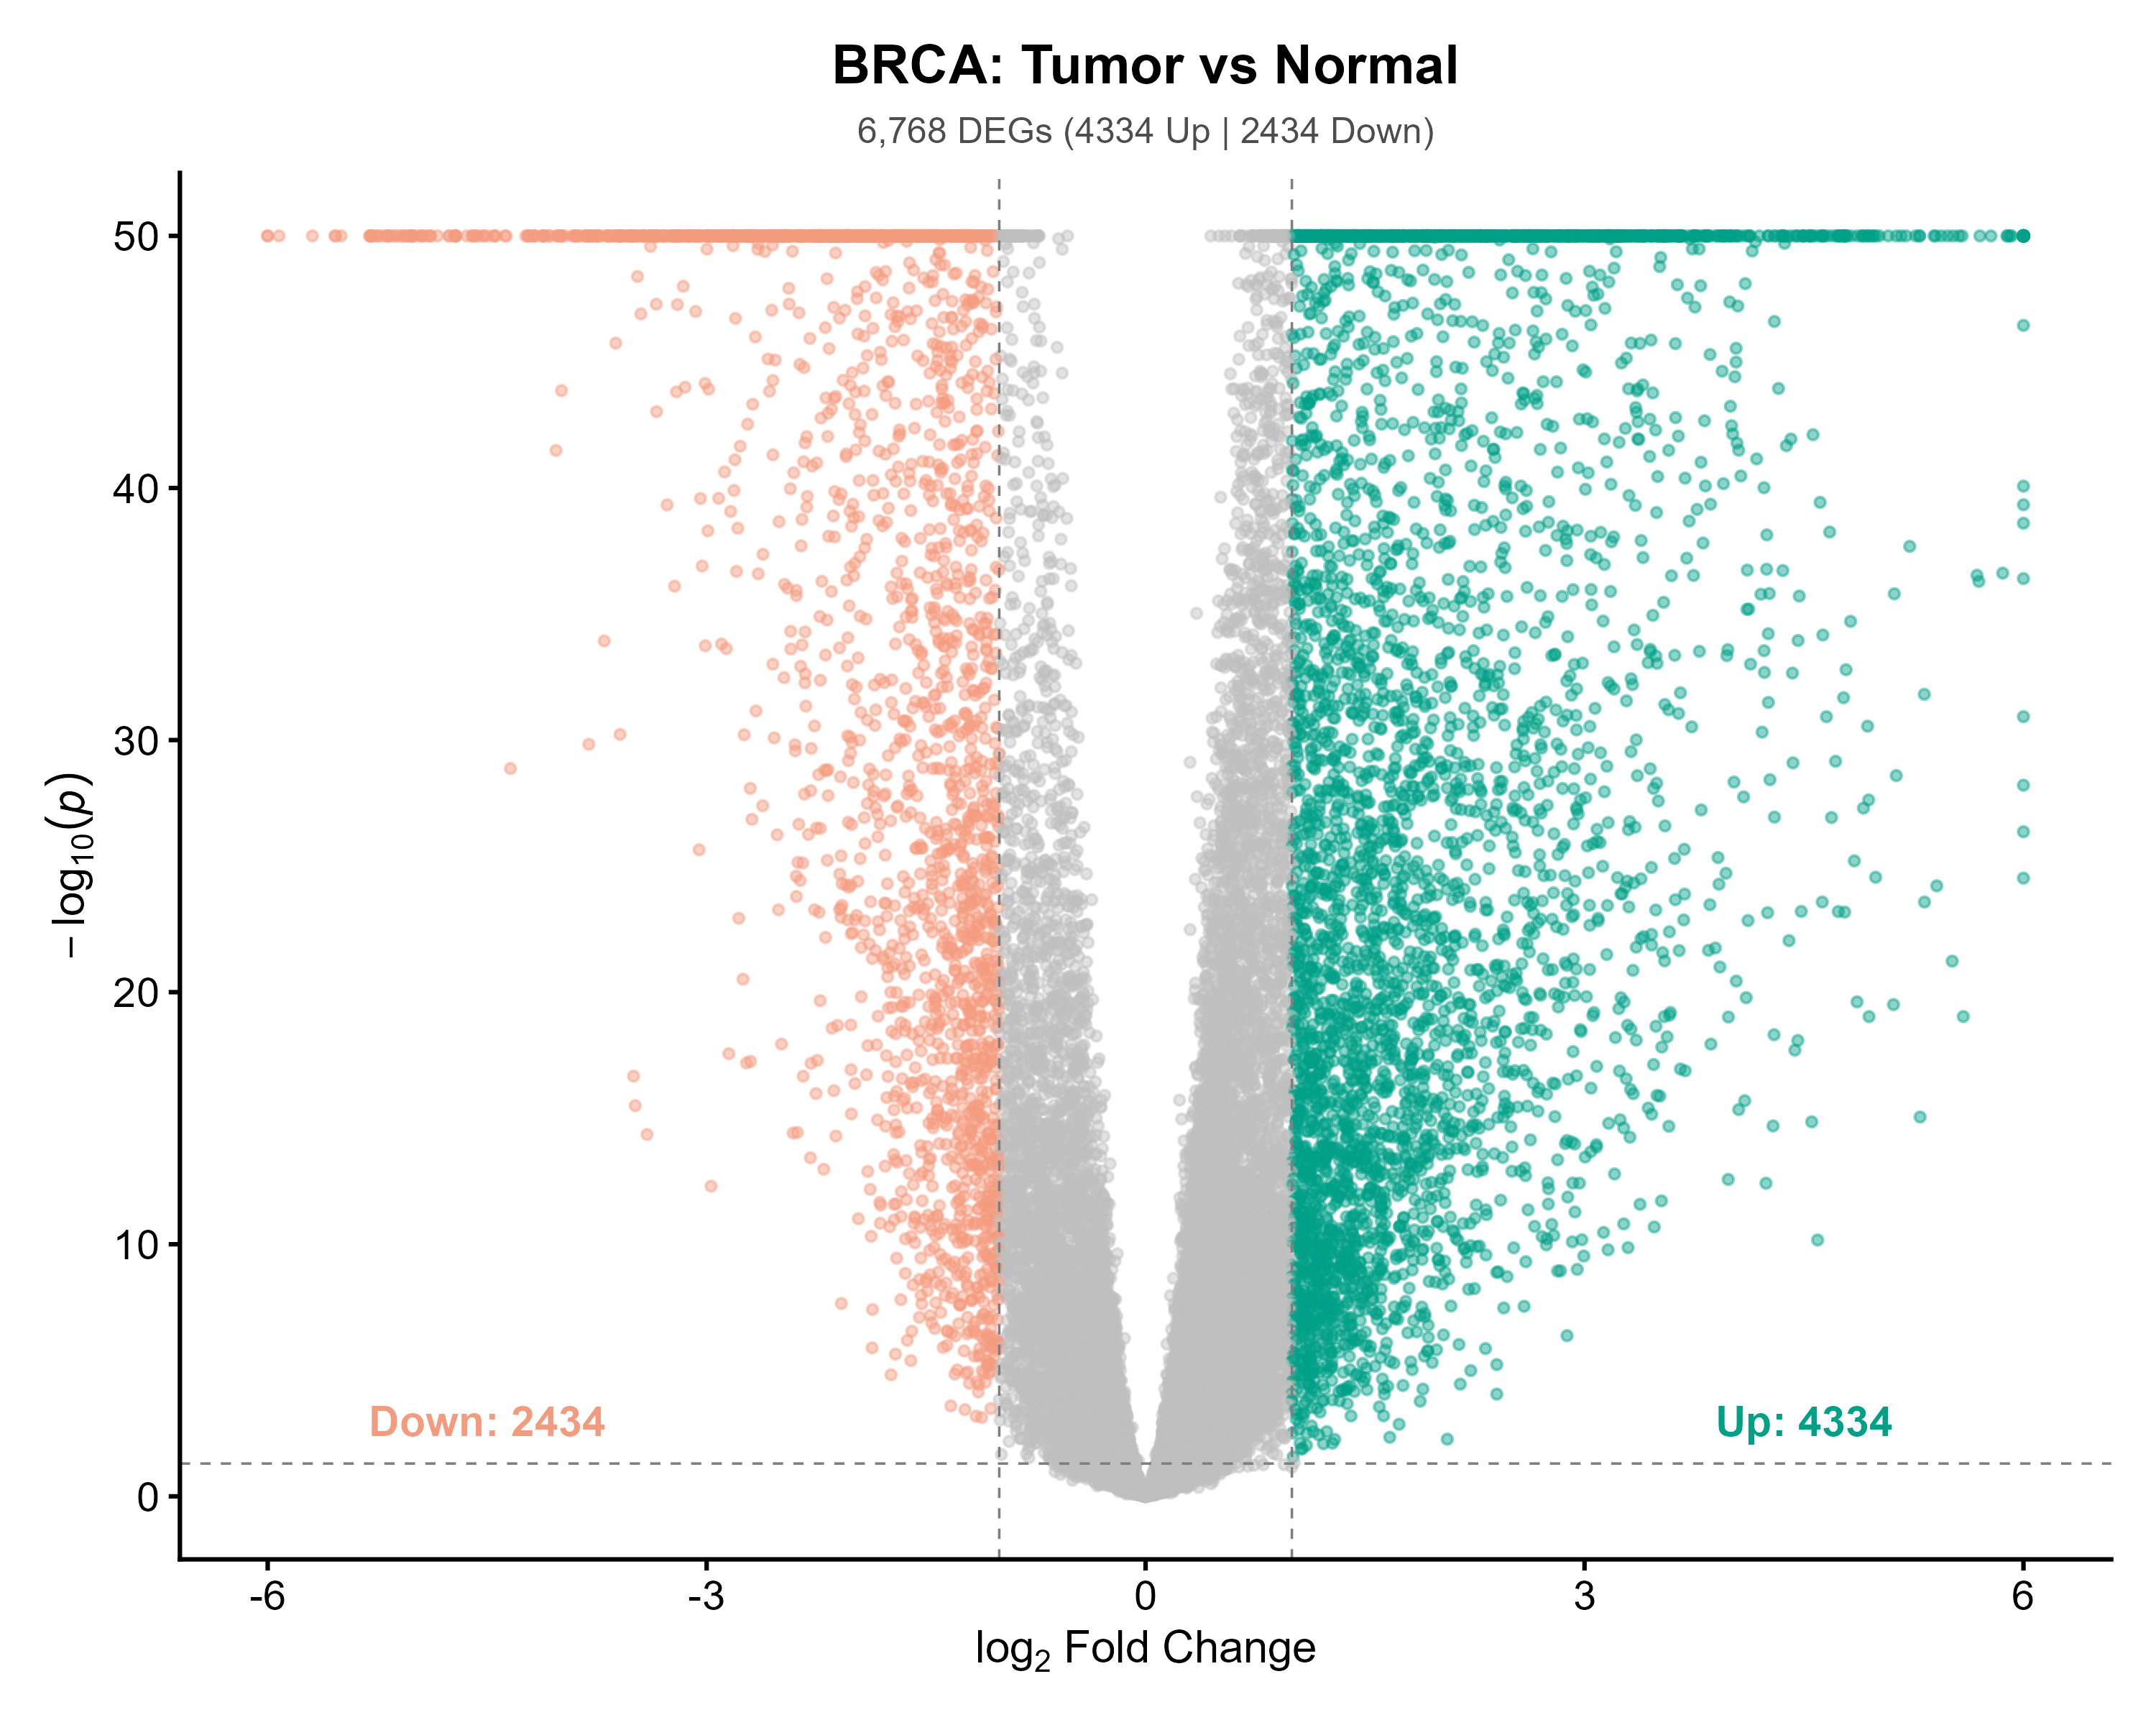
\includegraphics[width=0.85\textwidth]{fig1_volcano.png}
\caption{差异表达火山图（Tumor vs Normal, 6,768 DEGs）}
\label{fig:volcano}
\end{figure}

\begin{table}[htbp]
\centering
\caption{差异表达分析结果汇总}
\label{tab:deg_summary}
\begin{tabular}{ll}
\toprule
指标 & 数值 \\
\midrule
分析基因总数（过滤后） & 25,981 \\
肿瘤组样本数 & 1,105 \\
正常组样本数 & 113 \\
总DEGs（$|\log_2\text{FC}|>1$, FDR$<0.05$） & 6,768 \\
上调基因数 & 4,334 \\
下调基因数 & 2,434 \\
分析方法 & DESeq2 (Wald test, BH correction) \\
\bottomrule
\end{tabular}
\end{table}

\subsection{功能富集分析}

采用g:Profiler在线API（gprofiler2 R包）进行功能富集分析\cite{kolberg2023gprofiler}，覆盖GO、KEGG、Reactome和WikiPathway六个数据库（FDR$<0.05$）。分别对上调基因（4,334个）、下调基因（2,434个）和全部差异基因（6,768个）进行富集。

如图\ref{fig:enrich_up}所示，上调基因共富集到643条显著条目，富集信号高度集中——前五位通路全部来自Reactome：Cell Cycle（187个基因，$p=1.5\times10^{-21}$）、Cell Cycle Mitotic、Nucleosome Assembly、DNA Replication及Mitotic Chromosome Condensation。下调基因富集到1,414条显著条目（图\ref{fig:enrich_down}），集中于细胞外基质组织（ECM organization）、细胞黏附、脂质代谢和PI3K-Akt信号通路，条目数量超过上调基因的两倍（表\ref{tab:enrich_summary}）。

\begin{figure}[H]
\centering
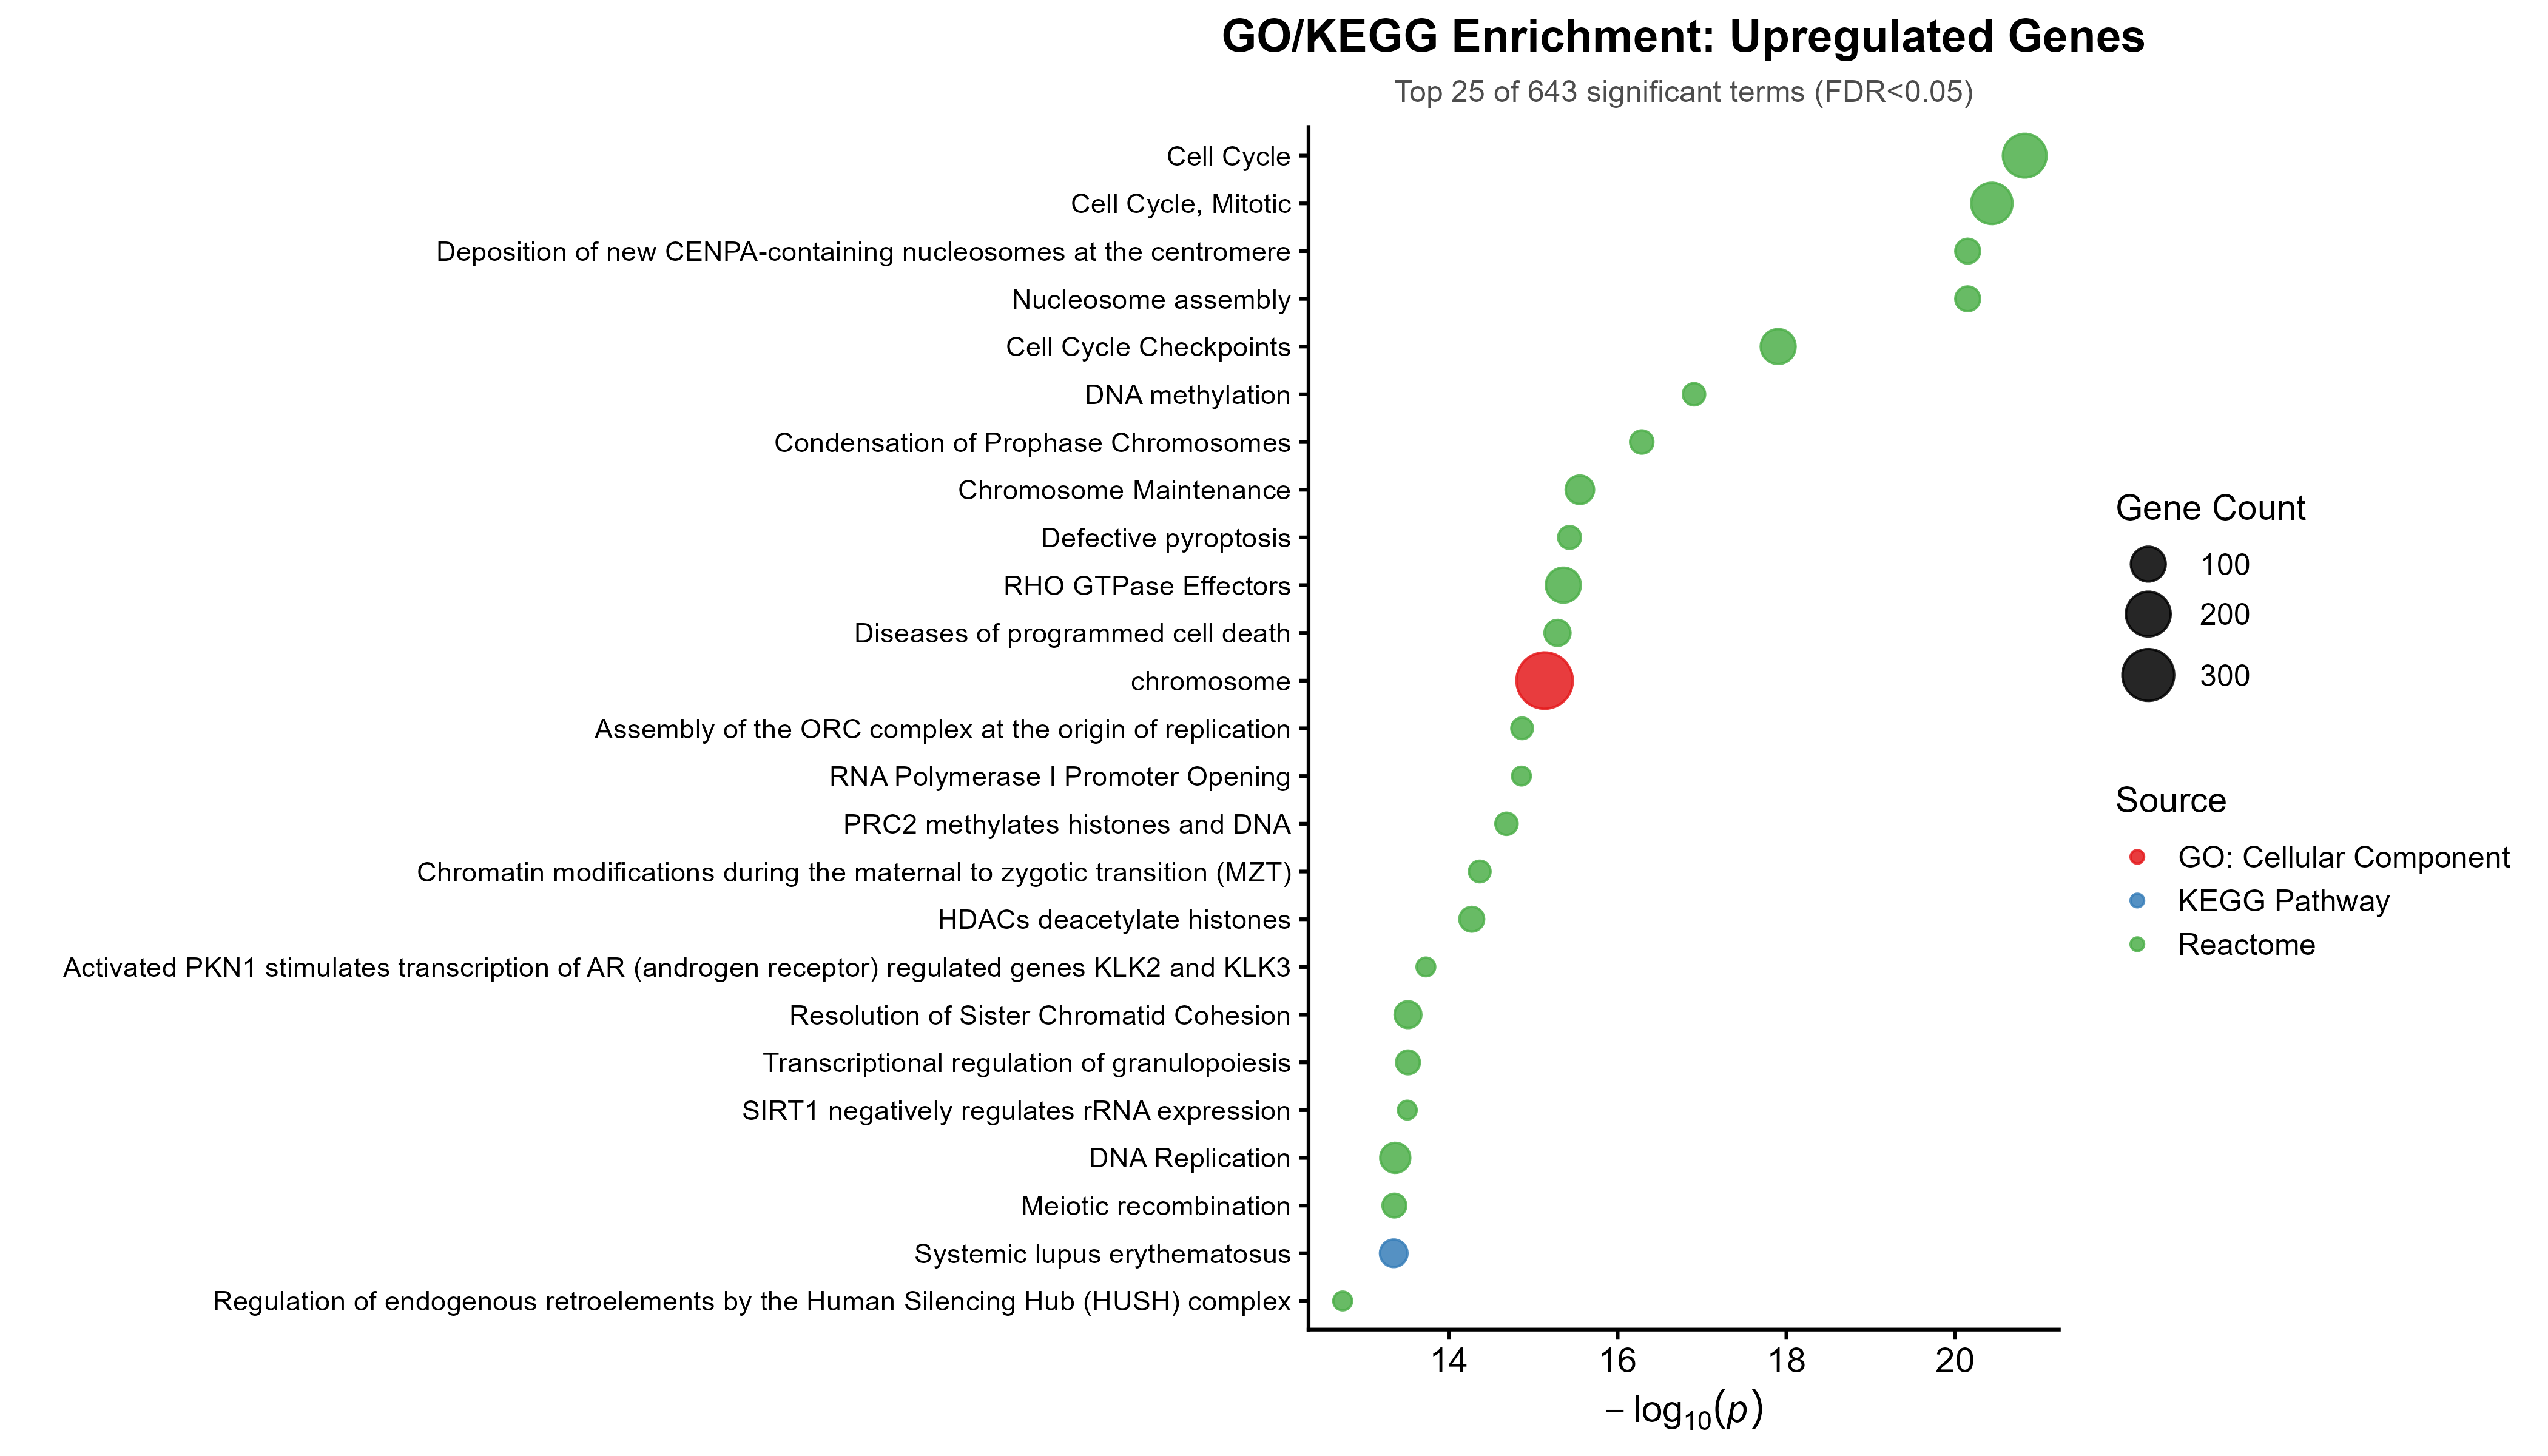
\includegraphics[width=0.85\textwidth]{fig12_enrichment_up.png}
\caption{上调基因GO/KEGG富集气泡图（Top 25, FDR$<0.05$）}
\label{fig:enrich_up}
\end{figure}

\begin{figure}[H]
\centering
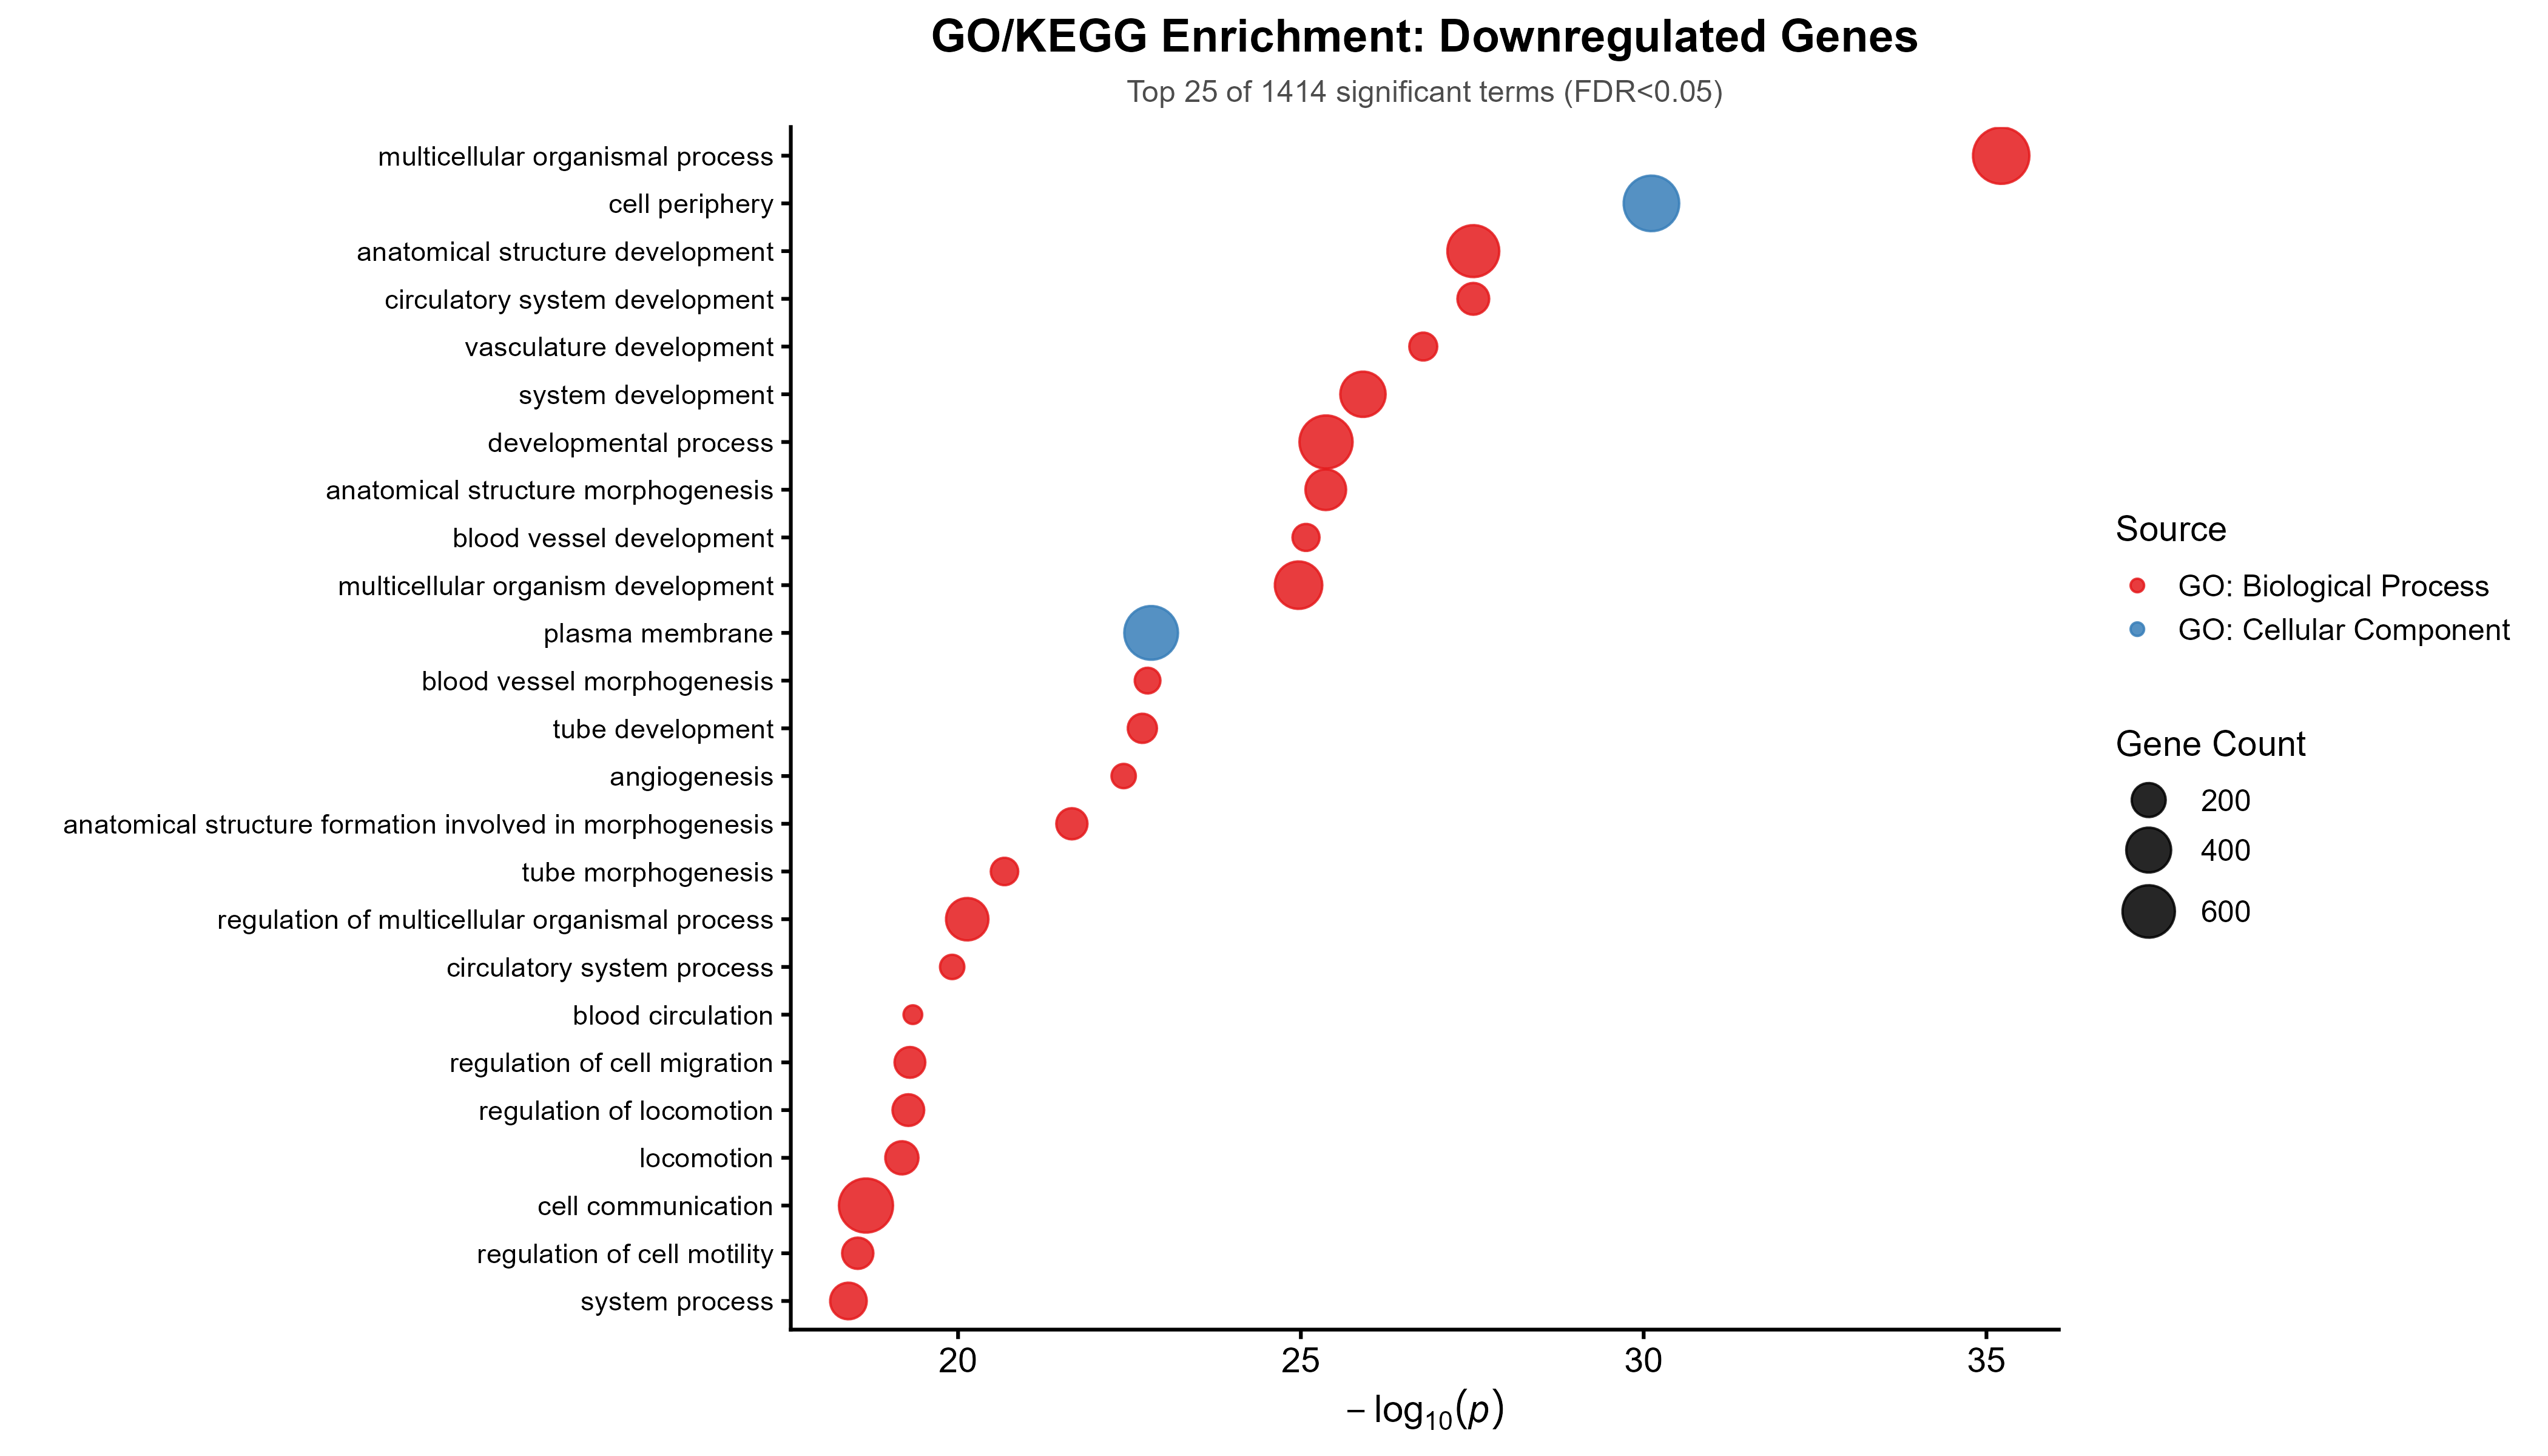
\includegraphics[width=0.85\textwidth]{fig13_enrichment_down.png}
\caption{下调基因富集气泡图（Top 25, FDR$<0.05$）}
\label{fig:enrich_down}
\end{figure}

\begin{table}[htbp]
\centering
\caption{功能富集分析结果汇总}
\label{tab:enrich_summary}
\begin{tabular}{lllll}
\toprule
基因集 & 基因数 & 显著条目数 & Top通路 & $p$值 \\
\midrule
上调 & 4,334 & 643 & Cell Cycle (Reactome) & $1.5\times10^{-21}$ \\
下调 & 2,434 & 1,414 & ECM Organization (Reactome) & $\sim10^{-15}$ \\
全部DEGs & 6,768 & 1,280 & Cell Cycle (Reactome) & $\sim10^{-18}$ \\
\bottomrule
\end{tabular}
\end{table}

\subsection{分子亚型分类}

比较LASSO多分类回归（5折交叉验证）、随机森林（ntree=500）和XGBoost（nrounds=100）三种算法对BRCA分子亚型的分类性能。输入特征为Top 500可变基因的$\log_2(\text{TPM}+1)$，训练集与测试集按7:3分层划分，分类标签为3类（Luminal A、HER2-enriched、Triple Negative）。

如图\ref{fig:model_comp}和表\ref{tab:class}所示，LASSO以89.4\%准确率（Kappa=0.528）居首，仅使用35个区分性基因，验证了亚型间转录组差异的稀疏性。随机森林以86.7\%（Kappa=0.365）次之。XGBoost准确率仅为35.8\%，主要因默认超参数未针对本数据调优。

\begin{figure}[H]
\centering
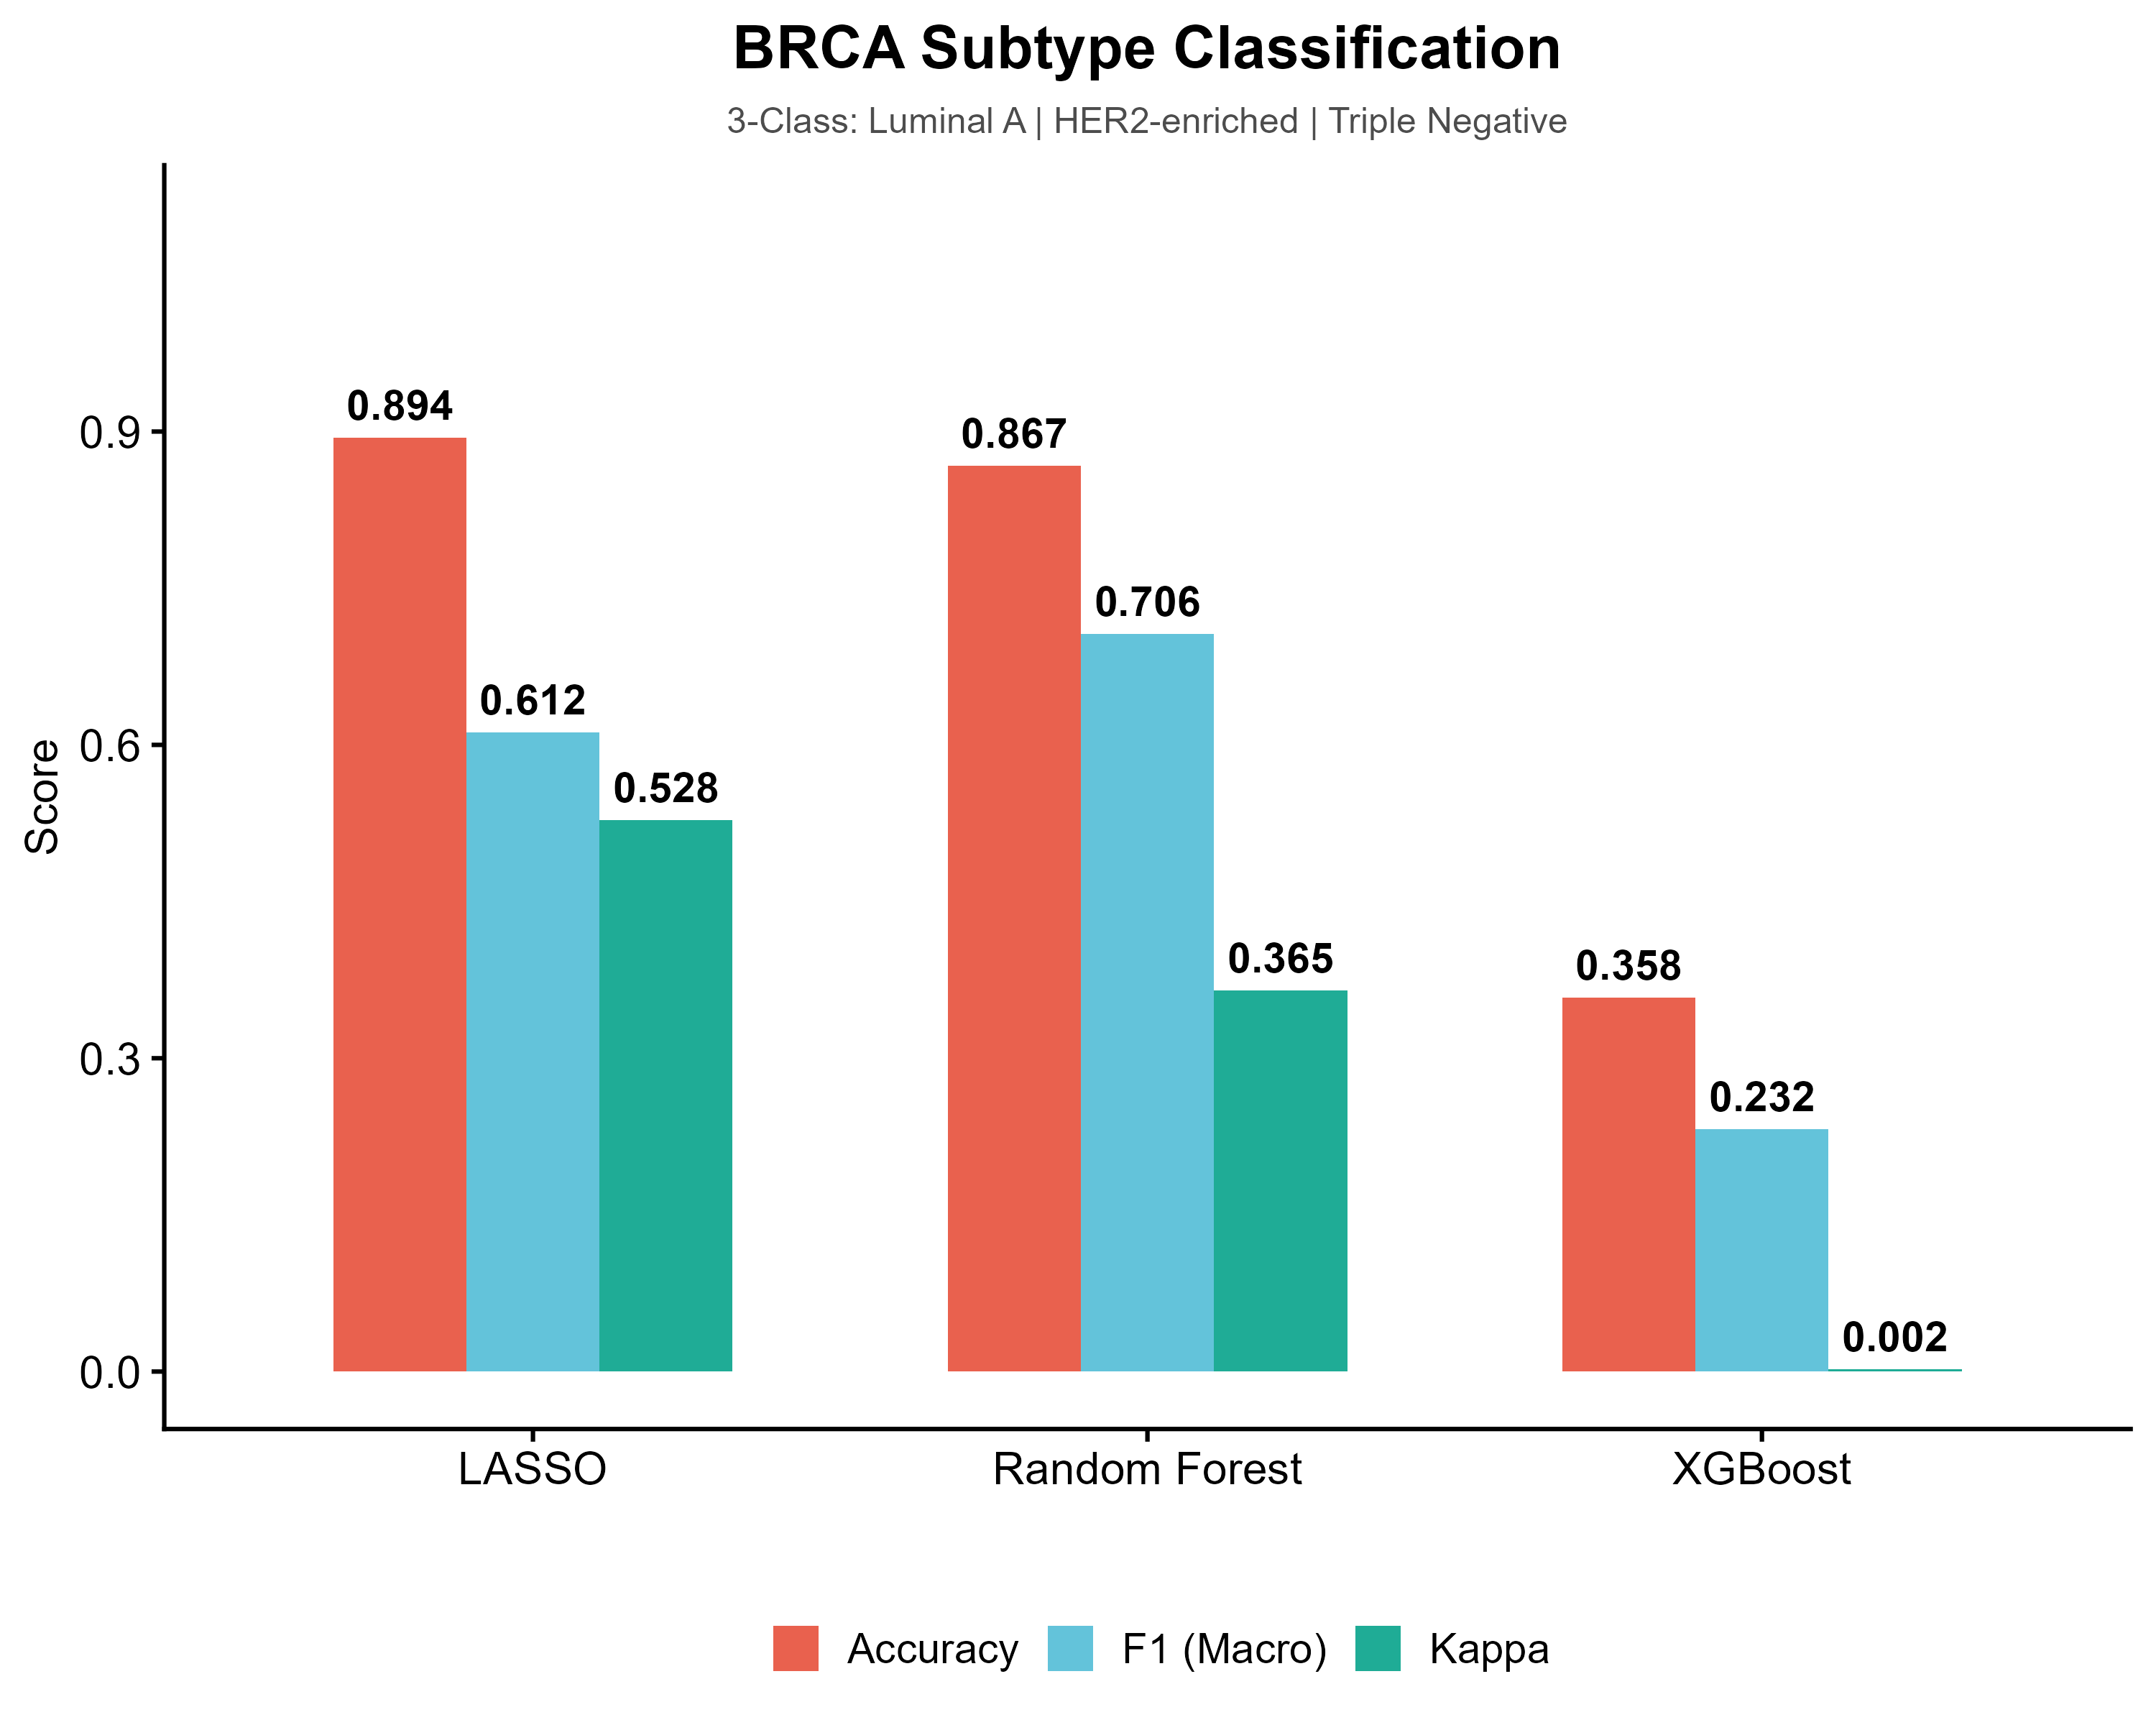
\includegraphics[width=0.7\textwidth]{fig6_model_comparison.png}
\caption{分子亚型分类模型性能对比（三指标分组柱状图）}
\label{fig:model_comp}
\end{figure}

\begin{table}[htbp]
\centering
\caption{分子亚型分类模型性能对比}
\label{tab:class}
\begin{tabular}{lllll}
\toprule
模型 & Accuracy & Kappa & F1 (Macro) & 特征数 \\
\midrule
LASSO (Multinomial) & 0.894 & 0.528 & 0.612 & 35 \\
Random Forest & 0.867 & 0.365 & 0.706 & 500 \\
XGBoost & 0.358 & 0.002 & 0.232 & 500 \\
\bottomrule
\end{tabular}
\end{table}

\subsection{聚类分析}

综合运用PCA、t-SNE、层次聚类、K-means及共识聚类五种方法探索BRCA转录组的自然分组结构。PCA对Top 2,000可变基因的$\log_2(\text{TPM}+1)$矩阵进行中心化和标准化。

如图\ref{fig:pca}所示，PC1（15.3\%）和PC2（8.5\%）合计解释了23.8\%的总方差。散点以NPG四色区分分子亚型，叠加95\%置信椭圆。Luminal A（绿色）形成紧凑簇，Triple Negative（红色）最为分散。PC1方向上的分离主要由ER状态驱动——ER+亚型（Luminal A/B）集中于负值侧，ER-亚型集中于正值侧。K-means轮廓系数在$K=2$时达到最大值0.18，支持ER+/ER-二分是BRCA转录组数据中最强的自然分组结构。

\begin{figure}[H]
\centering
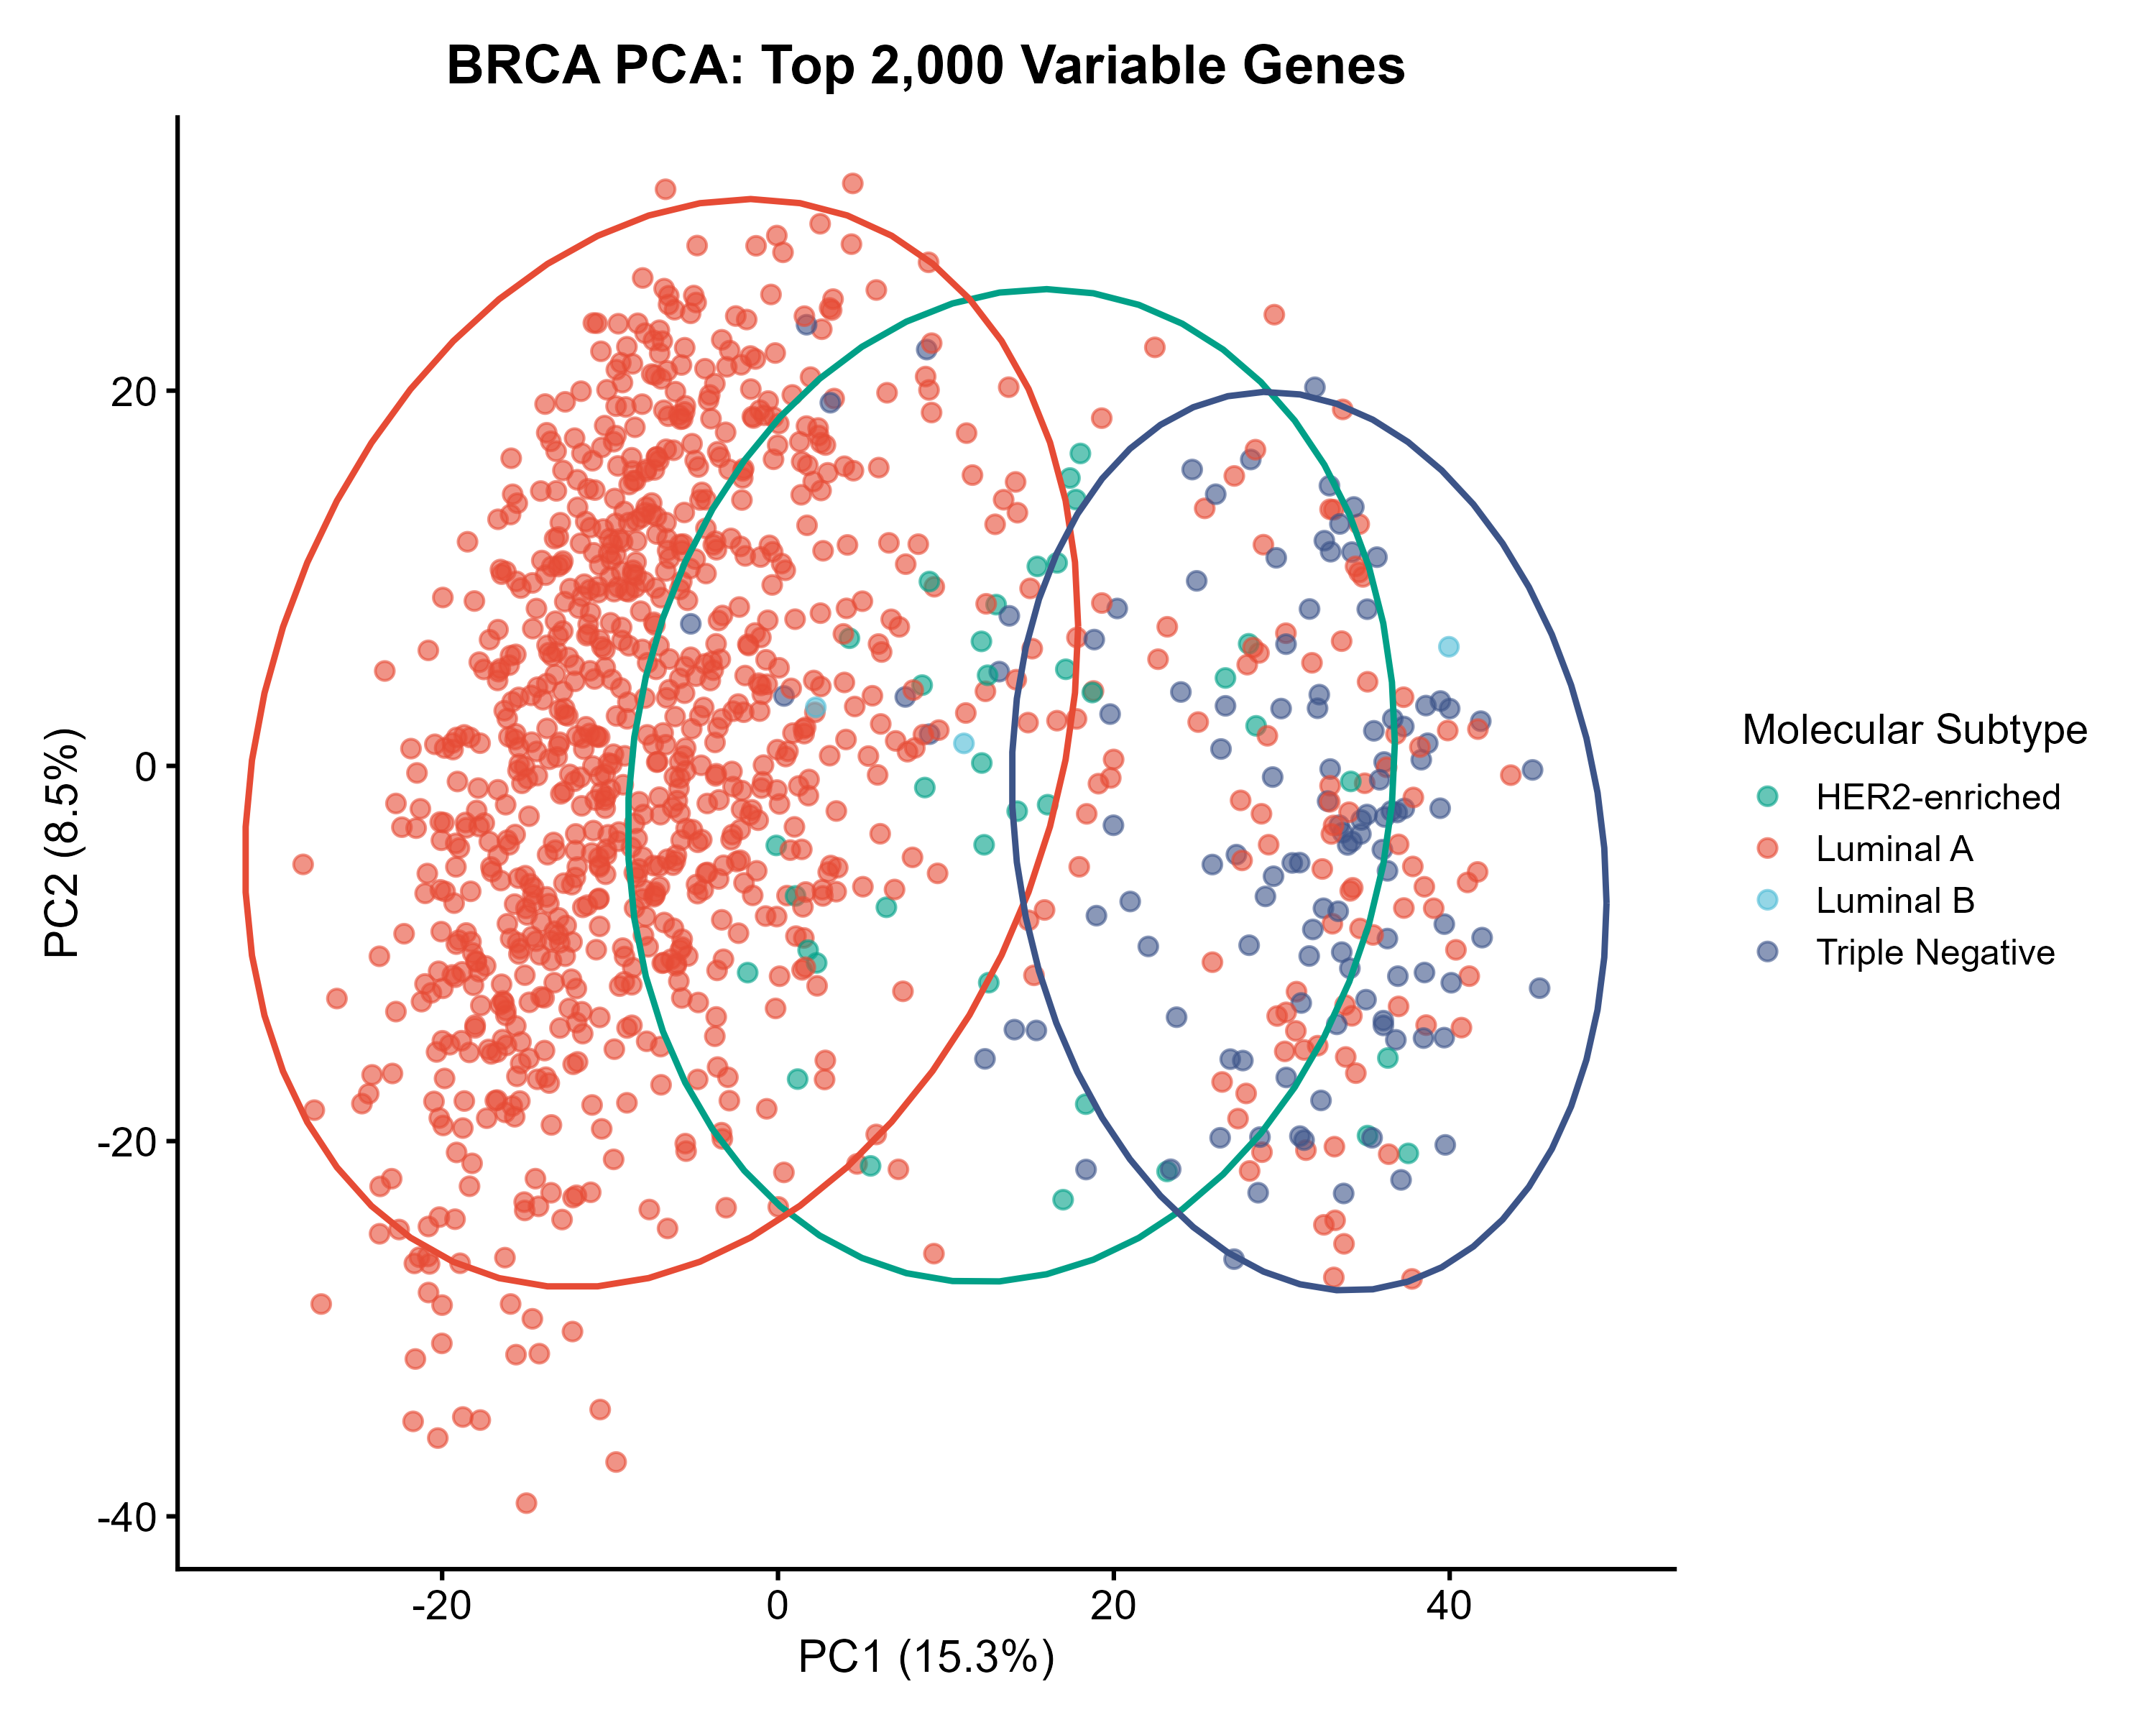
\includegraphics[width=0.85\textwidth]{fig2_pca_subtype.png}
\caption{PCA主成分分析（Top 2,000可变基因, PC1 15.3\% $\times$ PC2 8.5\%）}
\label{fig:pca}
\end{figure}

\subsection{WGCNA共表达网络分析}

使用Top 5,000可变基因在约1,100例肿瘤样本中的$\log_2(\text{TPM}+1)$矩阵进行WGCNA分析\cite{langfelder2008wgcna}。如图\ref{fig:wgcna_sft}所示，软阈值选择分析显示Power=8时达到scale-free $R^2=0.887$，同时平均连接度保持合理水平。

经动态树切割和相似模块合并后，共识别9个共表达模块（表\ref{tab:wgcna}）。不含grey（未分配模块，2,817个基因）的有效模块共8个，涵盖2,183个基因。Blue模块（553个基因）枢纽基因（ENSG00000167208）的模块内连接度$|\text{MM}|=0.959$为所有模块中最高。

\begin{figure}[H]
\centering
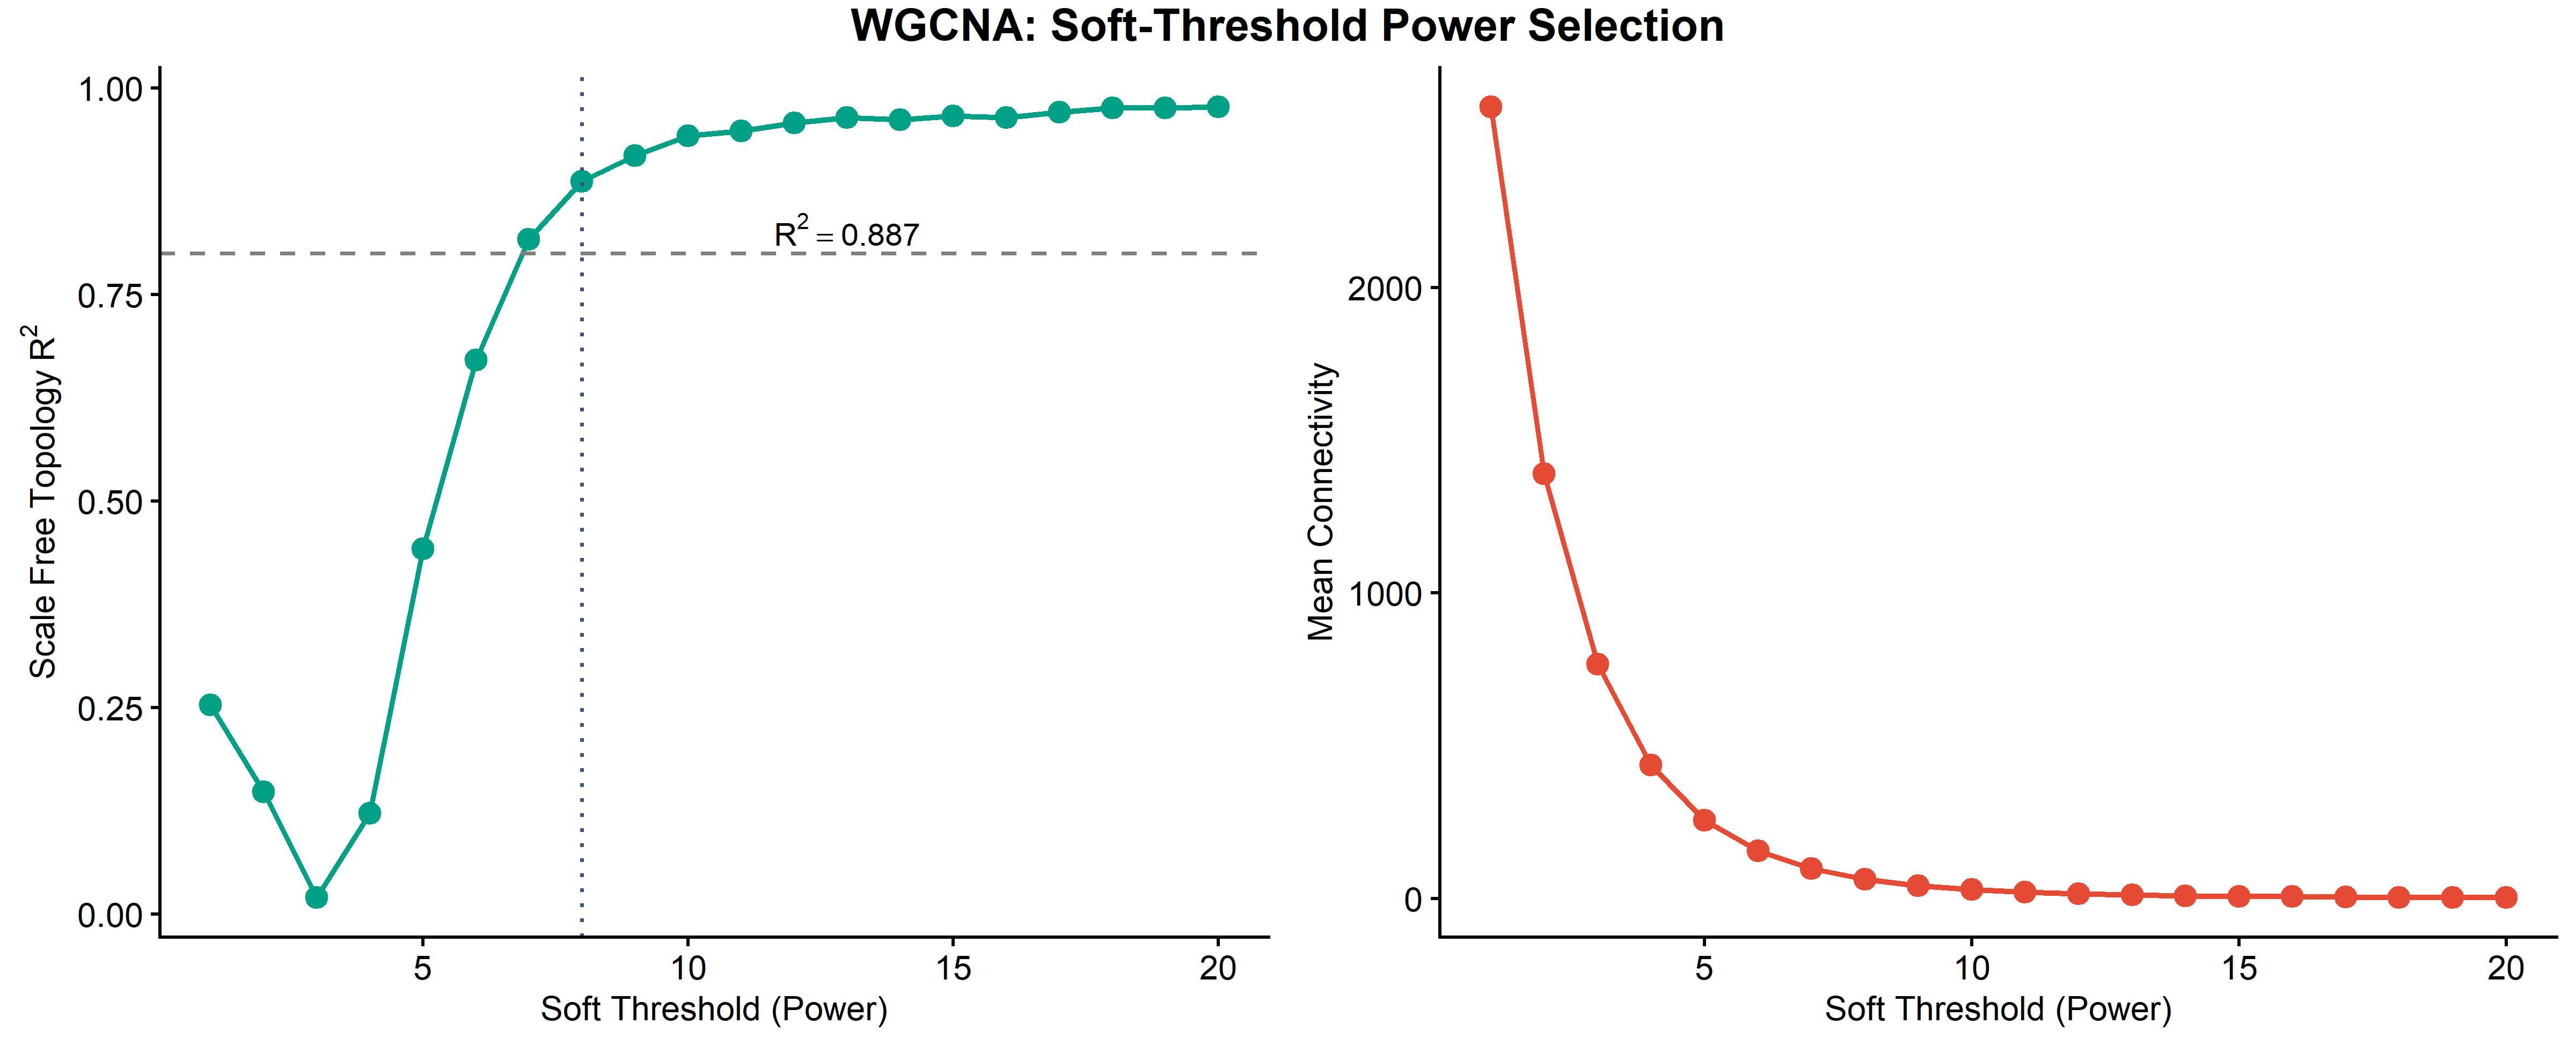
\includegraphics[width=0.95\textwidth]{fig7_wgcna_sft.png}
\caption{WGCNA软阈值选择（左：SFT $R^2$, 右：平均连接度）}
\label{fig:wgcna_sft}
\end{figure}

\begin{table}[htbp]
\centering
\caption{WGCNA共表达模块概况}
\label{tab:wgcna}
\begin{tabular}{llll}
\toprule
模块（颜色） & 基因数 & Top Hub Gene & $|\text{MM}|$ \\
\midrule
grey（未分配） & 2,817 & ENSG00000119866 & 0.836 \\
turquoise & 584 & ENSG00000115163 & 0.889 \\
\textbf{blue} & \textbf{553} & \textbf{ENSG00000167208} & \textbf{0.959} \\
brown & 336 & ENSG00000123500 & 0.911 \\
yellow & 260 & ENSG00000136997 & 0.874 \\
green & 224 & ENSG00000075624 & 0.903 \\
red & 119 & ENSG00000089157 & 0.881 \\
black & 63 & ENSG00000131143 & 0.854 \\
pink & 44 & ENSG00000117525 & 0.847 \\
\bottomrule
\end{tabular}
\end{table}

\subsection{生存分析}

采用Kaplan-Meier生存曲线和Cox比例风险回归评估临床及分子特征的预后价值。Cox模型纳入变量包括年龄、淋巴结阳性数、病理分期及分子亚型。

图\ref{fig:km}展示了按病理分期（I-IV）分层的KM曲线。四条曲线呈现清晰单调的逐级分离趋势（log-rank $p<0.0001$），附Number at Risk表展示各随访节点的存活样本数。多变量Cox回归森林图（图\ref{fig:cox}）显示Stage IV vs Stage I的风险比高达8.74（$95\%$CI: 3.61--21.14, $p<0.001$），Stage III的HR为2.96（$p=0.004$）。表\ref{tab:cox}详细列出各变量HR。Cox模型C-index为0.771（似然比$p=8.62\times10^{-12}$），证实病理分期是BRCA总生存的最强独立预测因子。

\begin{figure}[H]
\centering
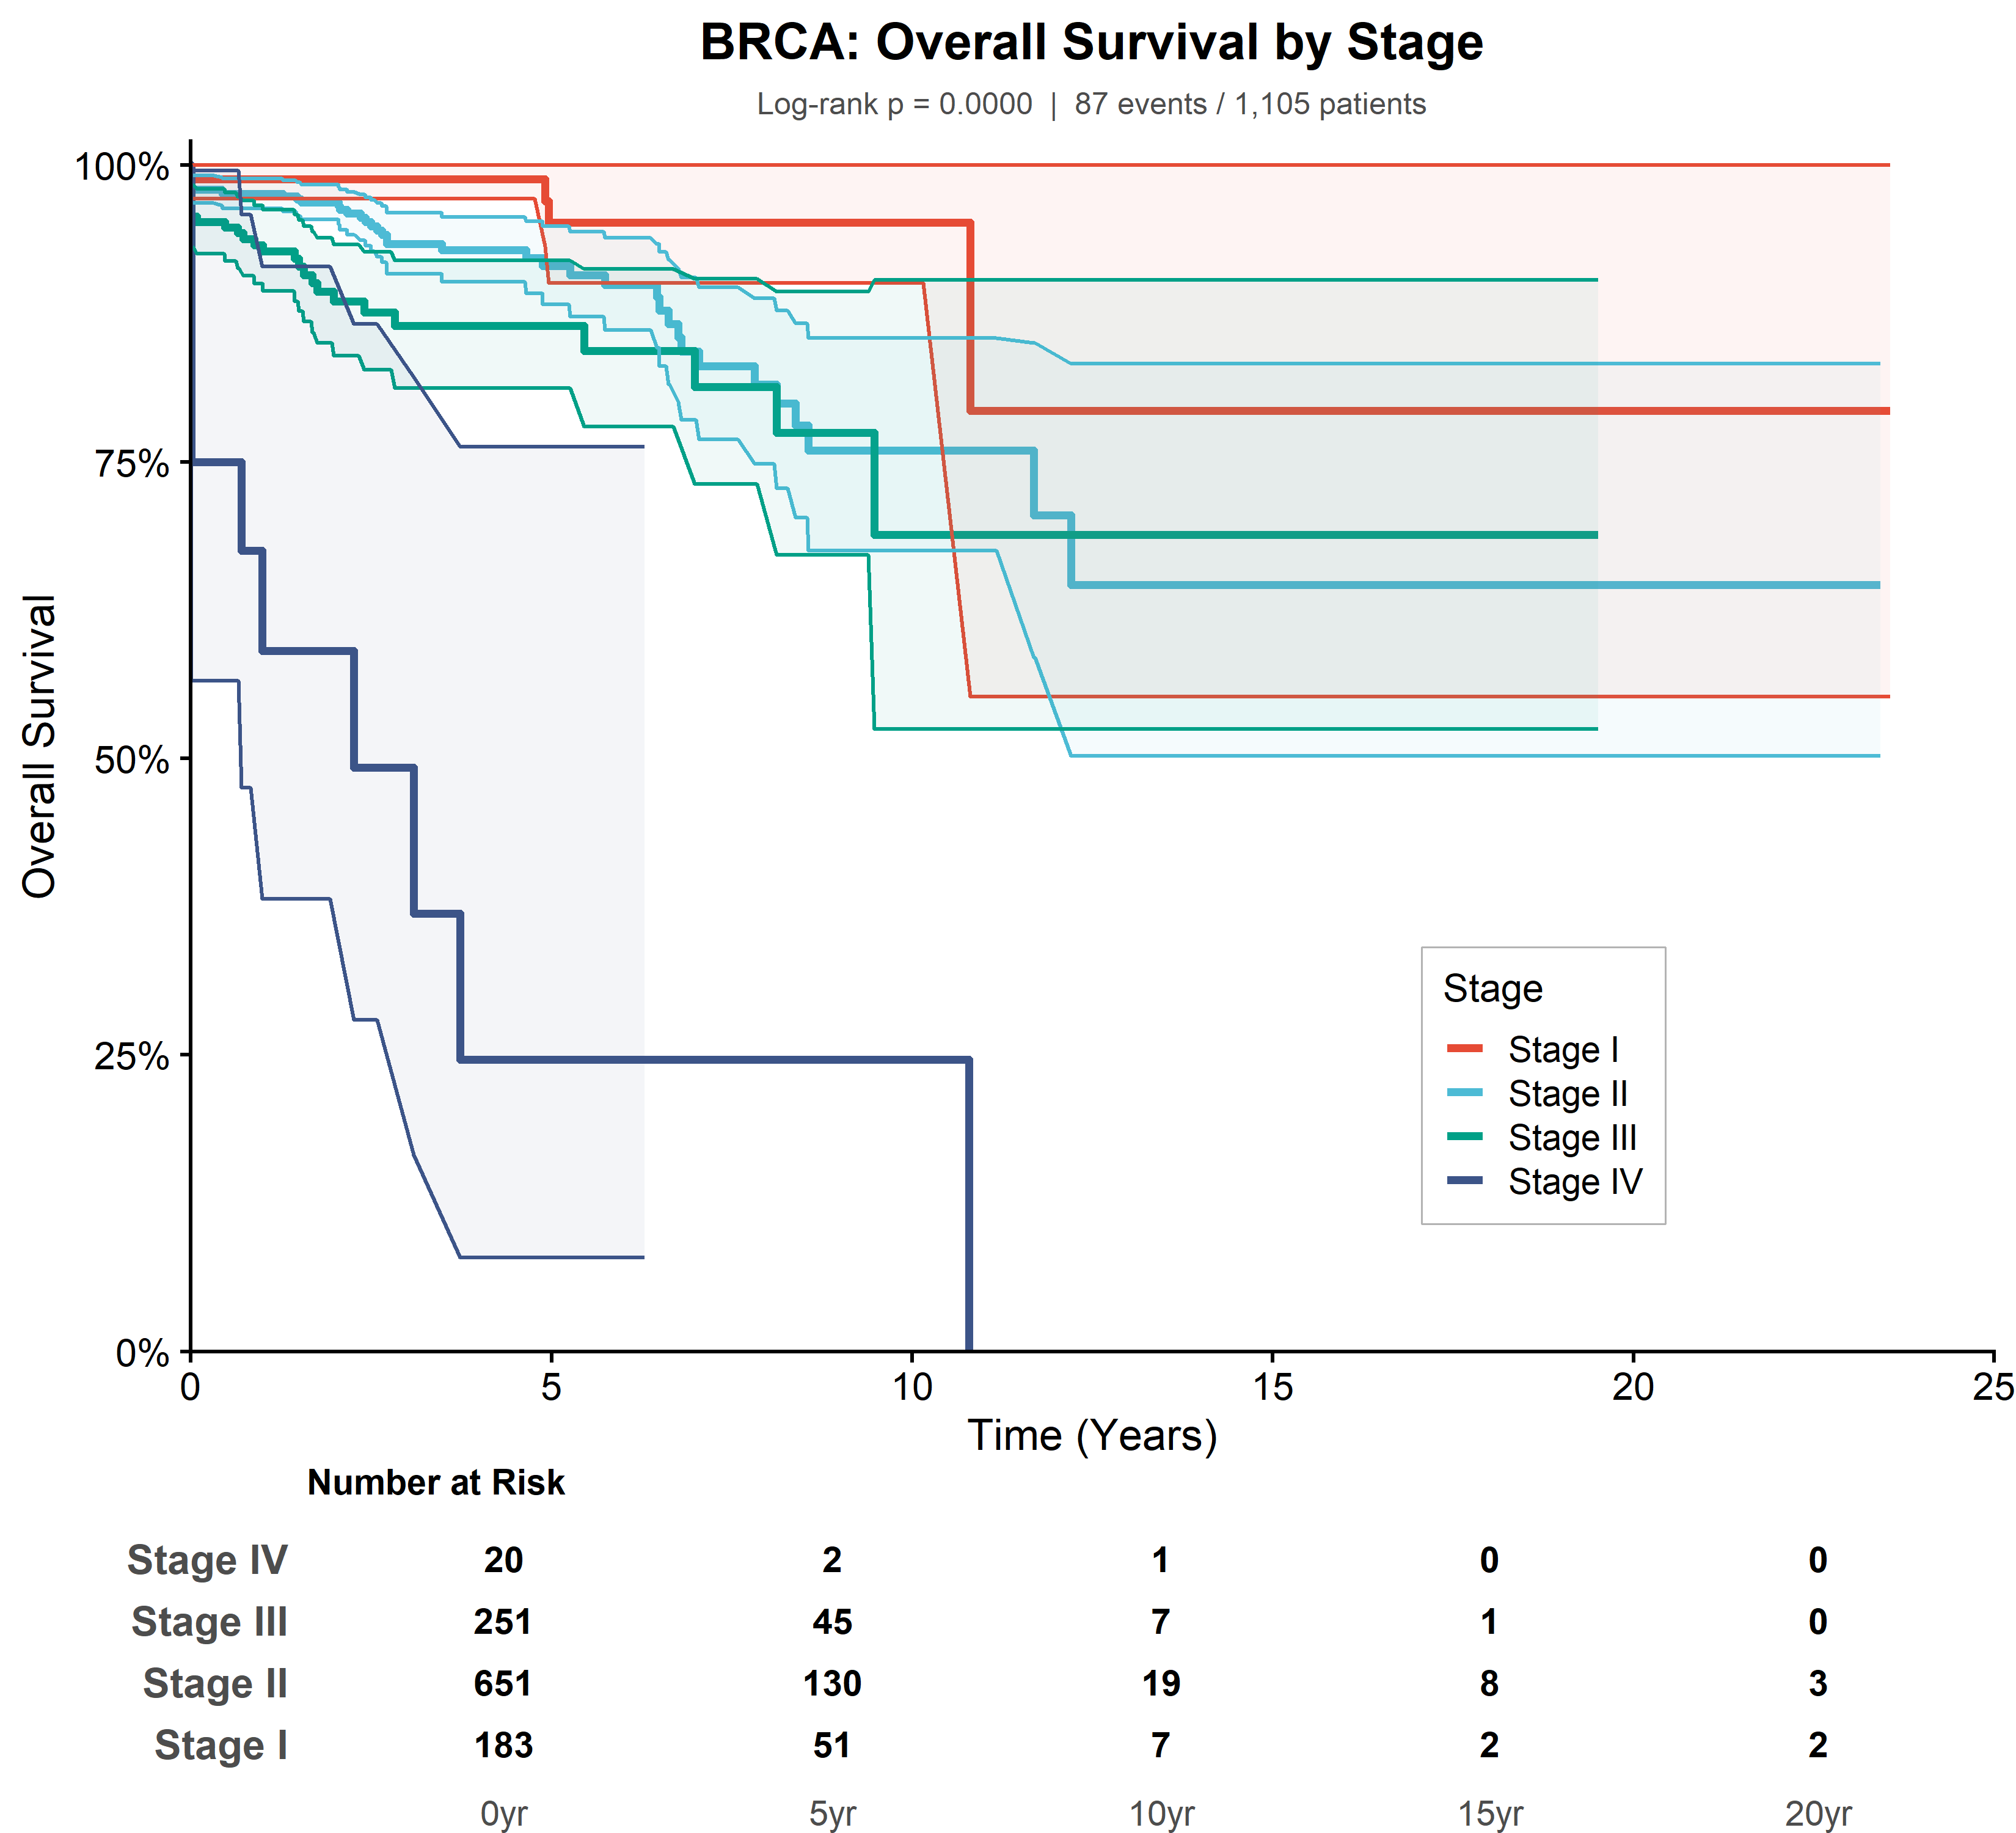
\includegraphics[width=0.85\textwidth]{fig3_km_stage.png}
\caption{Kaplan-Meier生存曲线（Stage I-IV, $p<0.0001$）}
\label{fig:km}
\end{figure}

\begin{figure}[H]
\centering
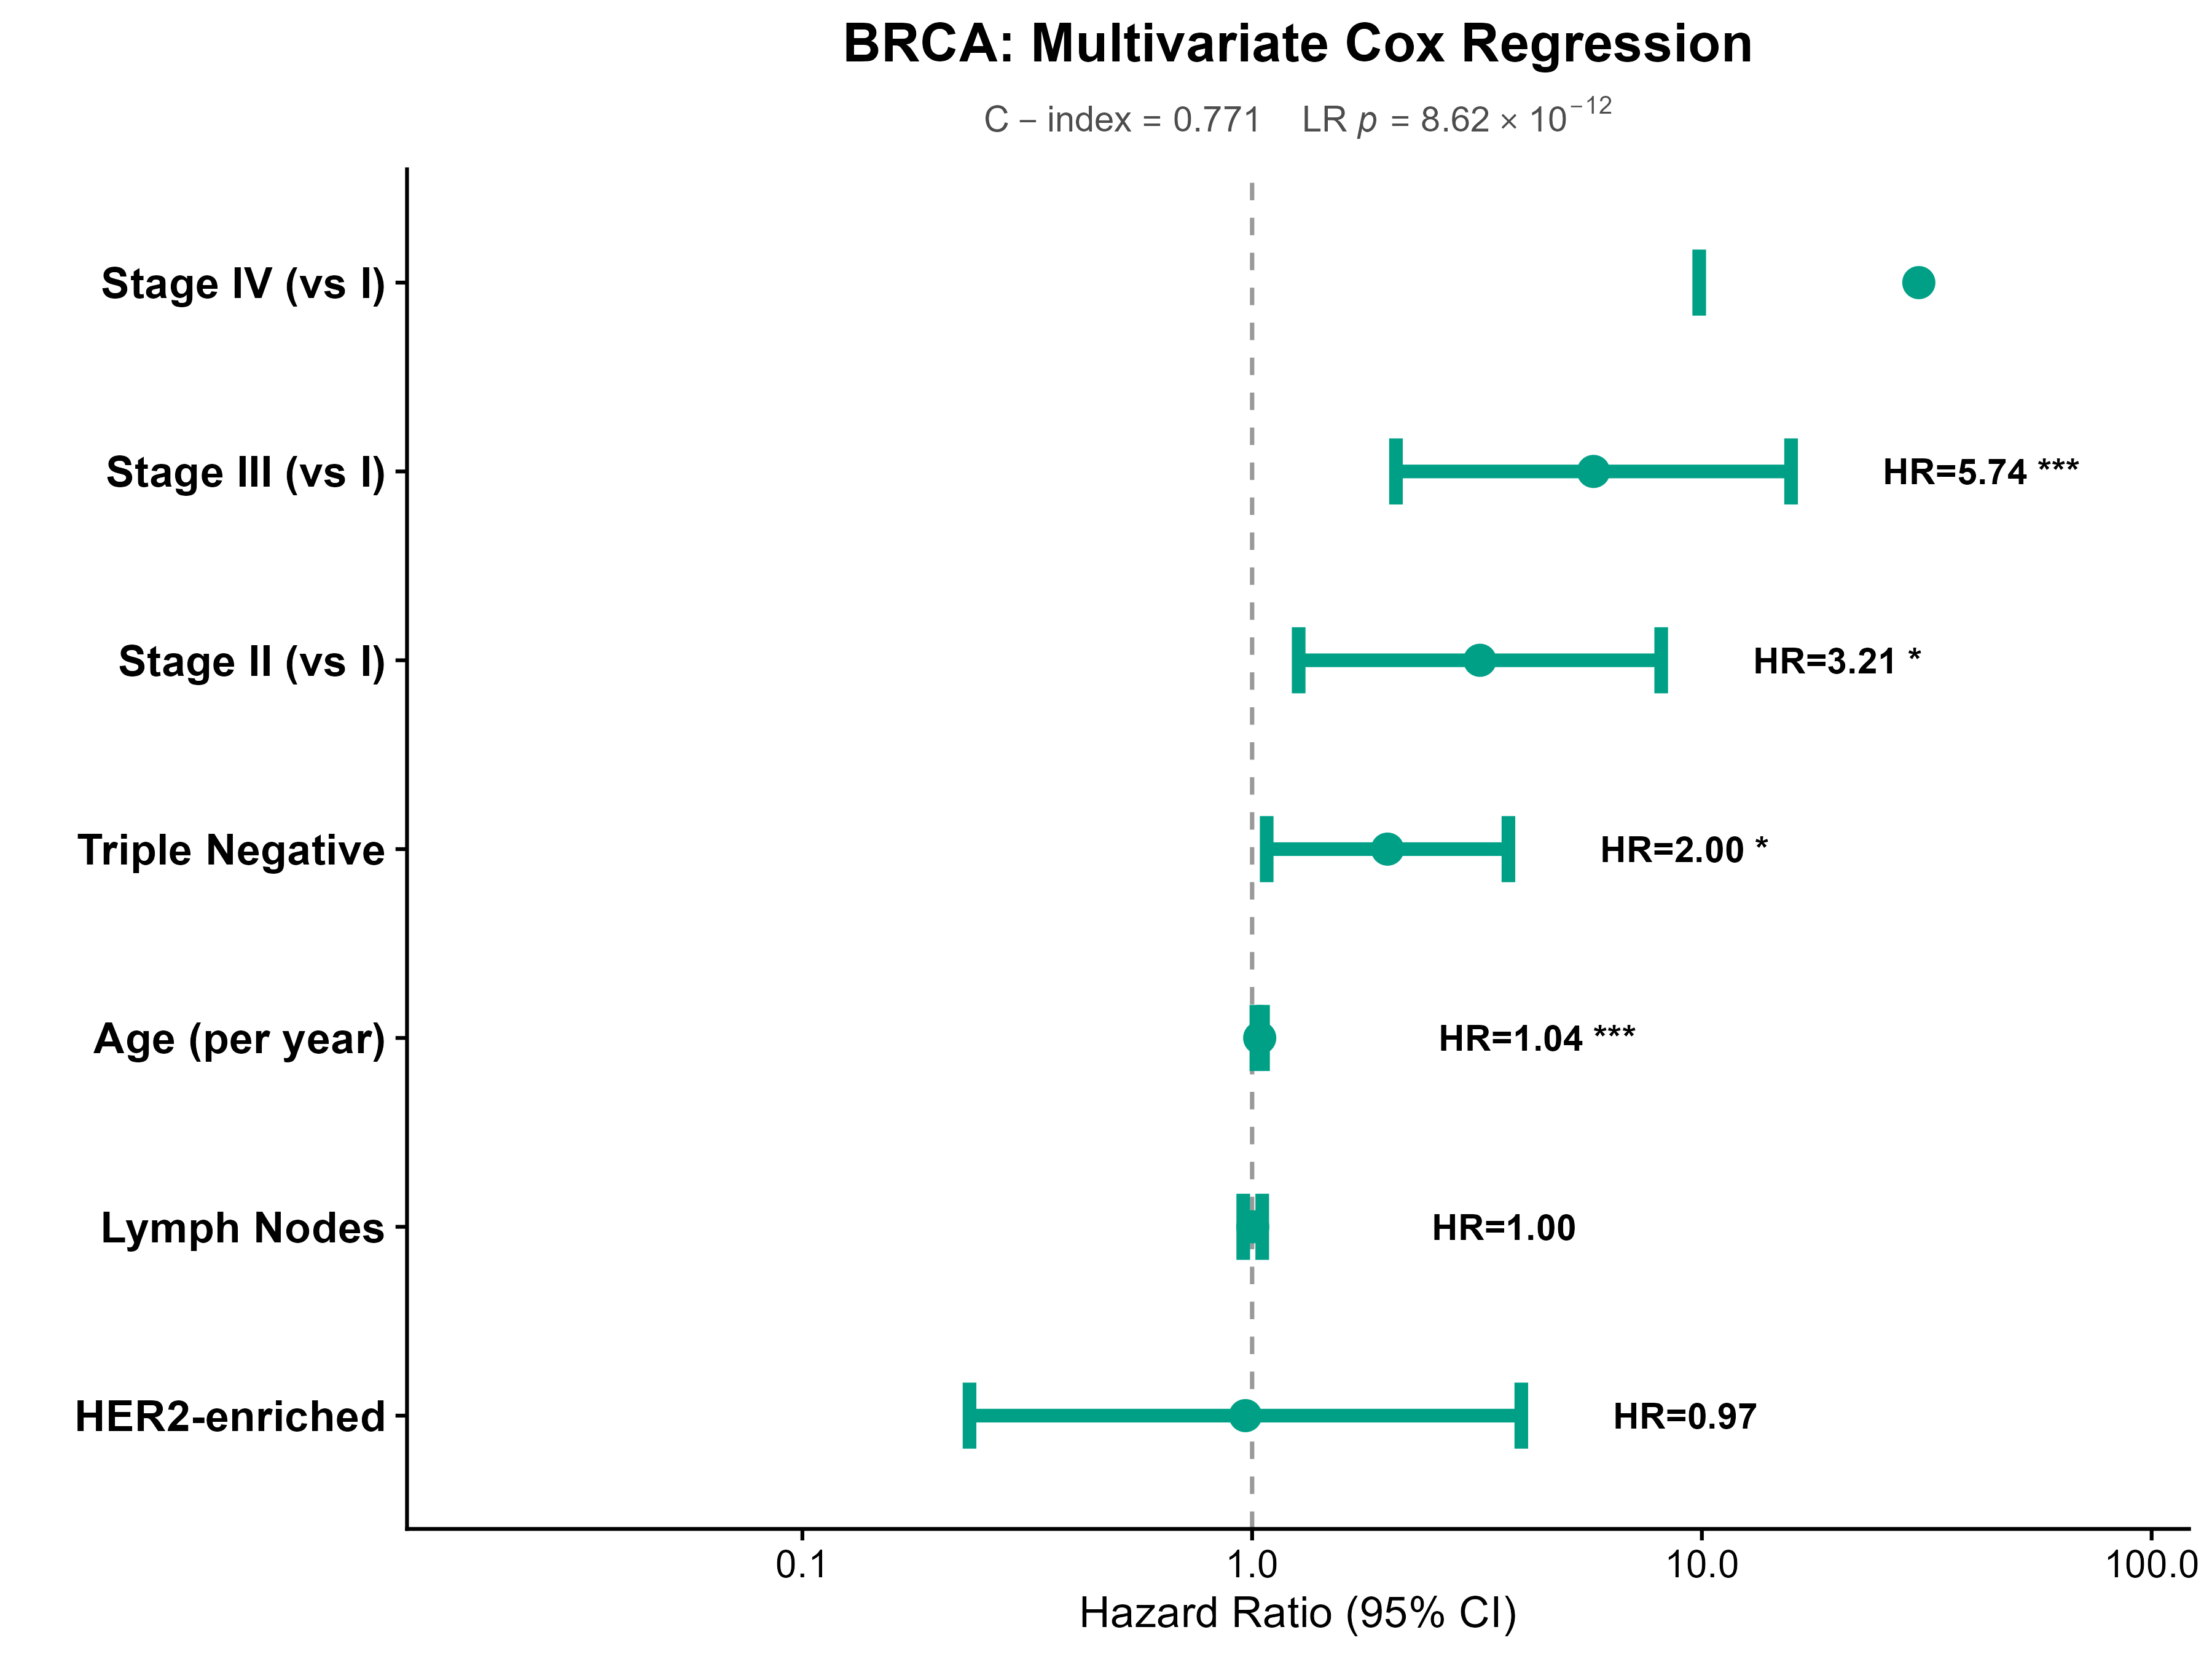
\includegraphics[width=0.85\textwidth]{fig9_cox_forest.png}
\caption{多变量Cox回归森林图（C-index=0.771）}
\label{fig:cox}
\end{figure}

\begin{table}[htbp]
\centering
\caption{多变量Cox回归结果（C-index=0.771）}
\label{tab:cox}
\begin{tabular}{lllll}
\toprule
变量 & HR & 95\% CI & $p$值 & 显著性 \\
\midrule
Age & 1.02 & 1.00--1.04 & 0.065 & \\
Lymph Nodes & 1.15 & 0.80--1.65 & 0.453 & \\
Stage II (vs I) & 1.82 & 0.99--3.35 & 0.054 & \\
Stage III (vs I) & 2.96 & 1.43--6.12 & 0.004 & ** \\
Stage IV (vs I) & 8.74 & 3.61--21.14 & $<0.001$ & *** \\
HER2-enriched & 1.21 & 0.62--2.36 & 0.578 & \\
Triple Negative & 1.02 & 0.57--1.82 & 0.947 & \\
\bottomrule
\end{tabular}
\end{table}

\subsection{体细胞突变分析}

采用maftools R包\cite{mayakonda2018maftools}对990例样本的体细胞突变数据进行系统分析。突变数据集涵盖15,413个突变基因、67,546个变异位点，平均每例约68个突变。

图\ref{fig:oncoplot}展示了Top 12突变基因的瀑布图。PIK3CA（369例，37.3\%）和TP53（348例，35.2\%）的突变频率远高于其他基因。TTN居第三位（268例，27.1\%），其高频突变部分归因于基因长度效应。表\ref{tab:mutation}列出Top 10突变基因。PIK3CA与TP53之间呈现互斥趋势，符合两种基因分别驱动不同信号通路的生物学逻辑。

\begin{figure}[H]
\centering
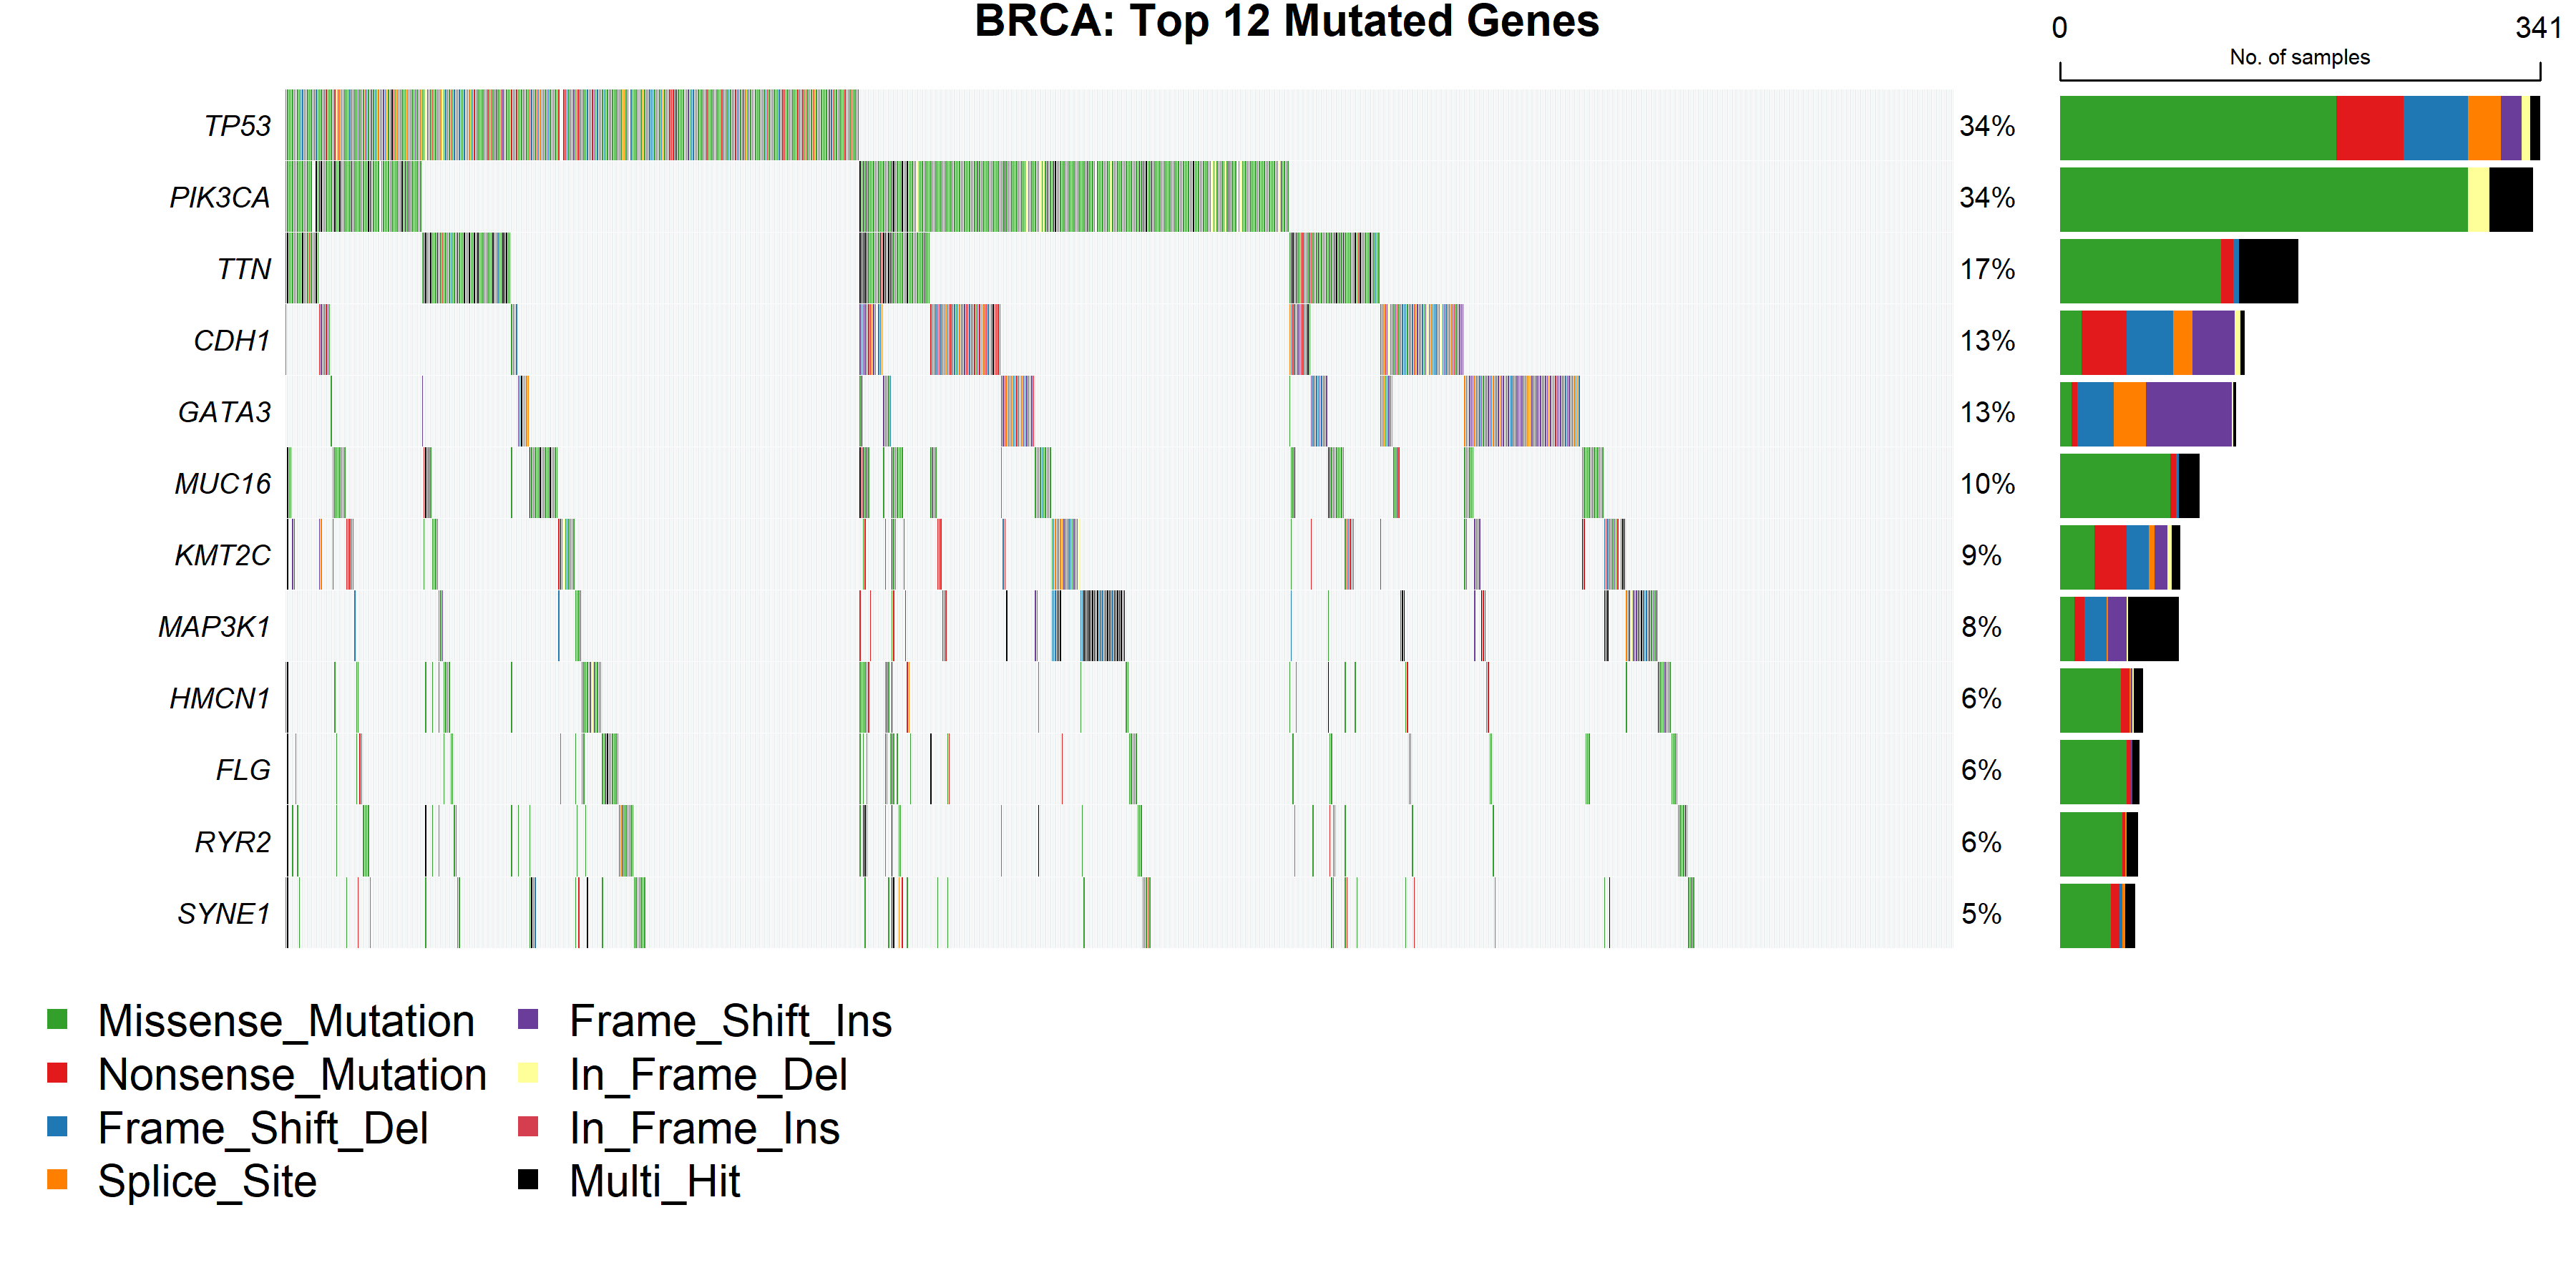
\includegraphics[width=\textwidth]{fig4_oncoplot.png}
\caption{体细胞突变瀑布图（Top 12基因, 990例样本）}
\label{fig:oncoplot}
\end{figure}

\begin{table}[htbp]
\centering
\caption{BRCA Top 10高频突变基因}
\label{tab:mutation}
\begin{tabular}{llll}
\toprule
排名 & 基因 & 突变样本数（频率） & 已知功能 \\
\midrule
1 & PIK3CA & 369 (37.3\%) & PI3K/AKT通路激活 \\
2 & TP53 & 348 (35.2\%) & 肿瘤抑制基因失活 \\
3 & TTN & 268 (27.1\%) & 肌联蛋白（乘客突变可能） \\
4 & CDH1 & 164 (16.6\%) & 细胞黏附 \\
5 & GATA3 & 148 (14.9\%) & 管腔分化转录因子 \\
6 & MUC16 & 131 (13.2\%) & 黏蛋白 \\
7 & MAP3K1 & 119 (12.0\%) & MAPK信号通路 \\
8 & KMT2C & 107 (10.8\%) & 组蛋白甲基转移酶 \\
9 & RYR2 & 98 (9.9\%) & 钙离子通道 \\
10 & FLG & 93 (9.4\%) & 表皮结构蛋白 \\
\bottomrule
\end{tabular}
\end{table}

\subsection{关联规则与调控网络}

采用Apriori算法（arules包）对基因表达高/低状态与临床特征之间的关联规则进行挖掘。图\ref{fig:rules}以散点图展示关联规则的全局分布：横轴为Support，纵轴为Confidence，点的大小和颜色编码Lift值。

miRNA-mRNA调控网络通过Pearson相关矩阵构建。图\ref{fig:mirna}为Top 20 miRNA-mRNA调控对的相关性热图，以红-白-蓝渐变色阶编码相关系数。以$|r|>0.4$为阈值共识别2,065对显著调控关系对。

\begin{figure}[H]
\centering
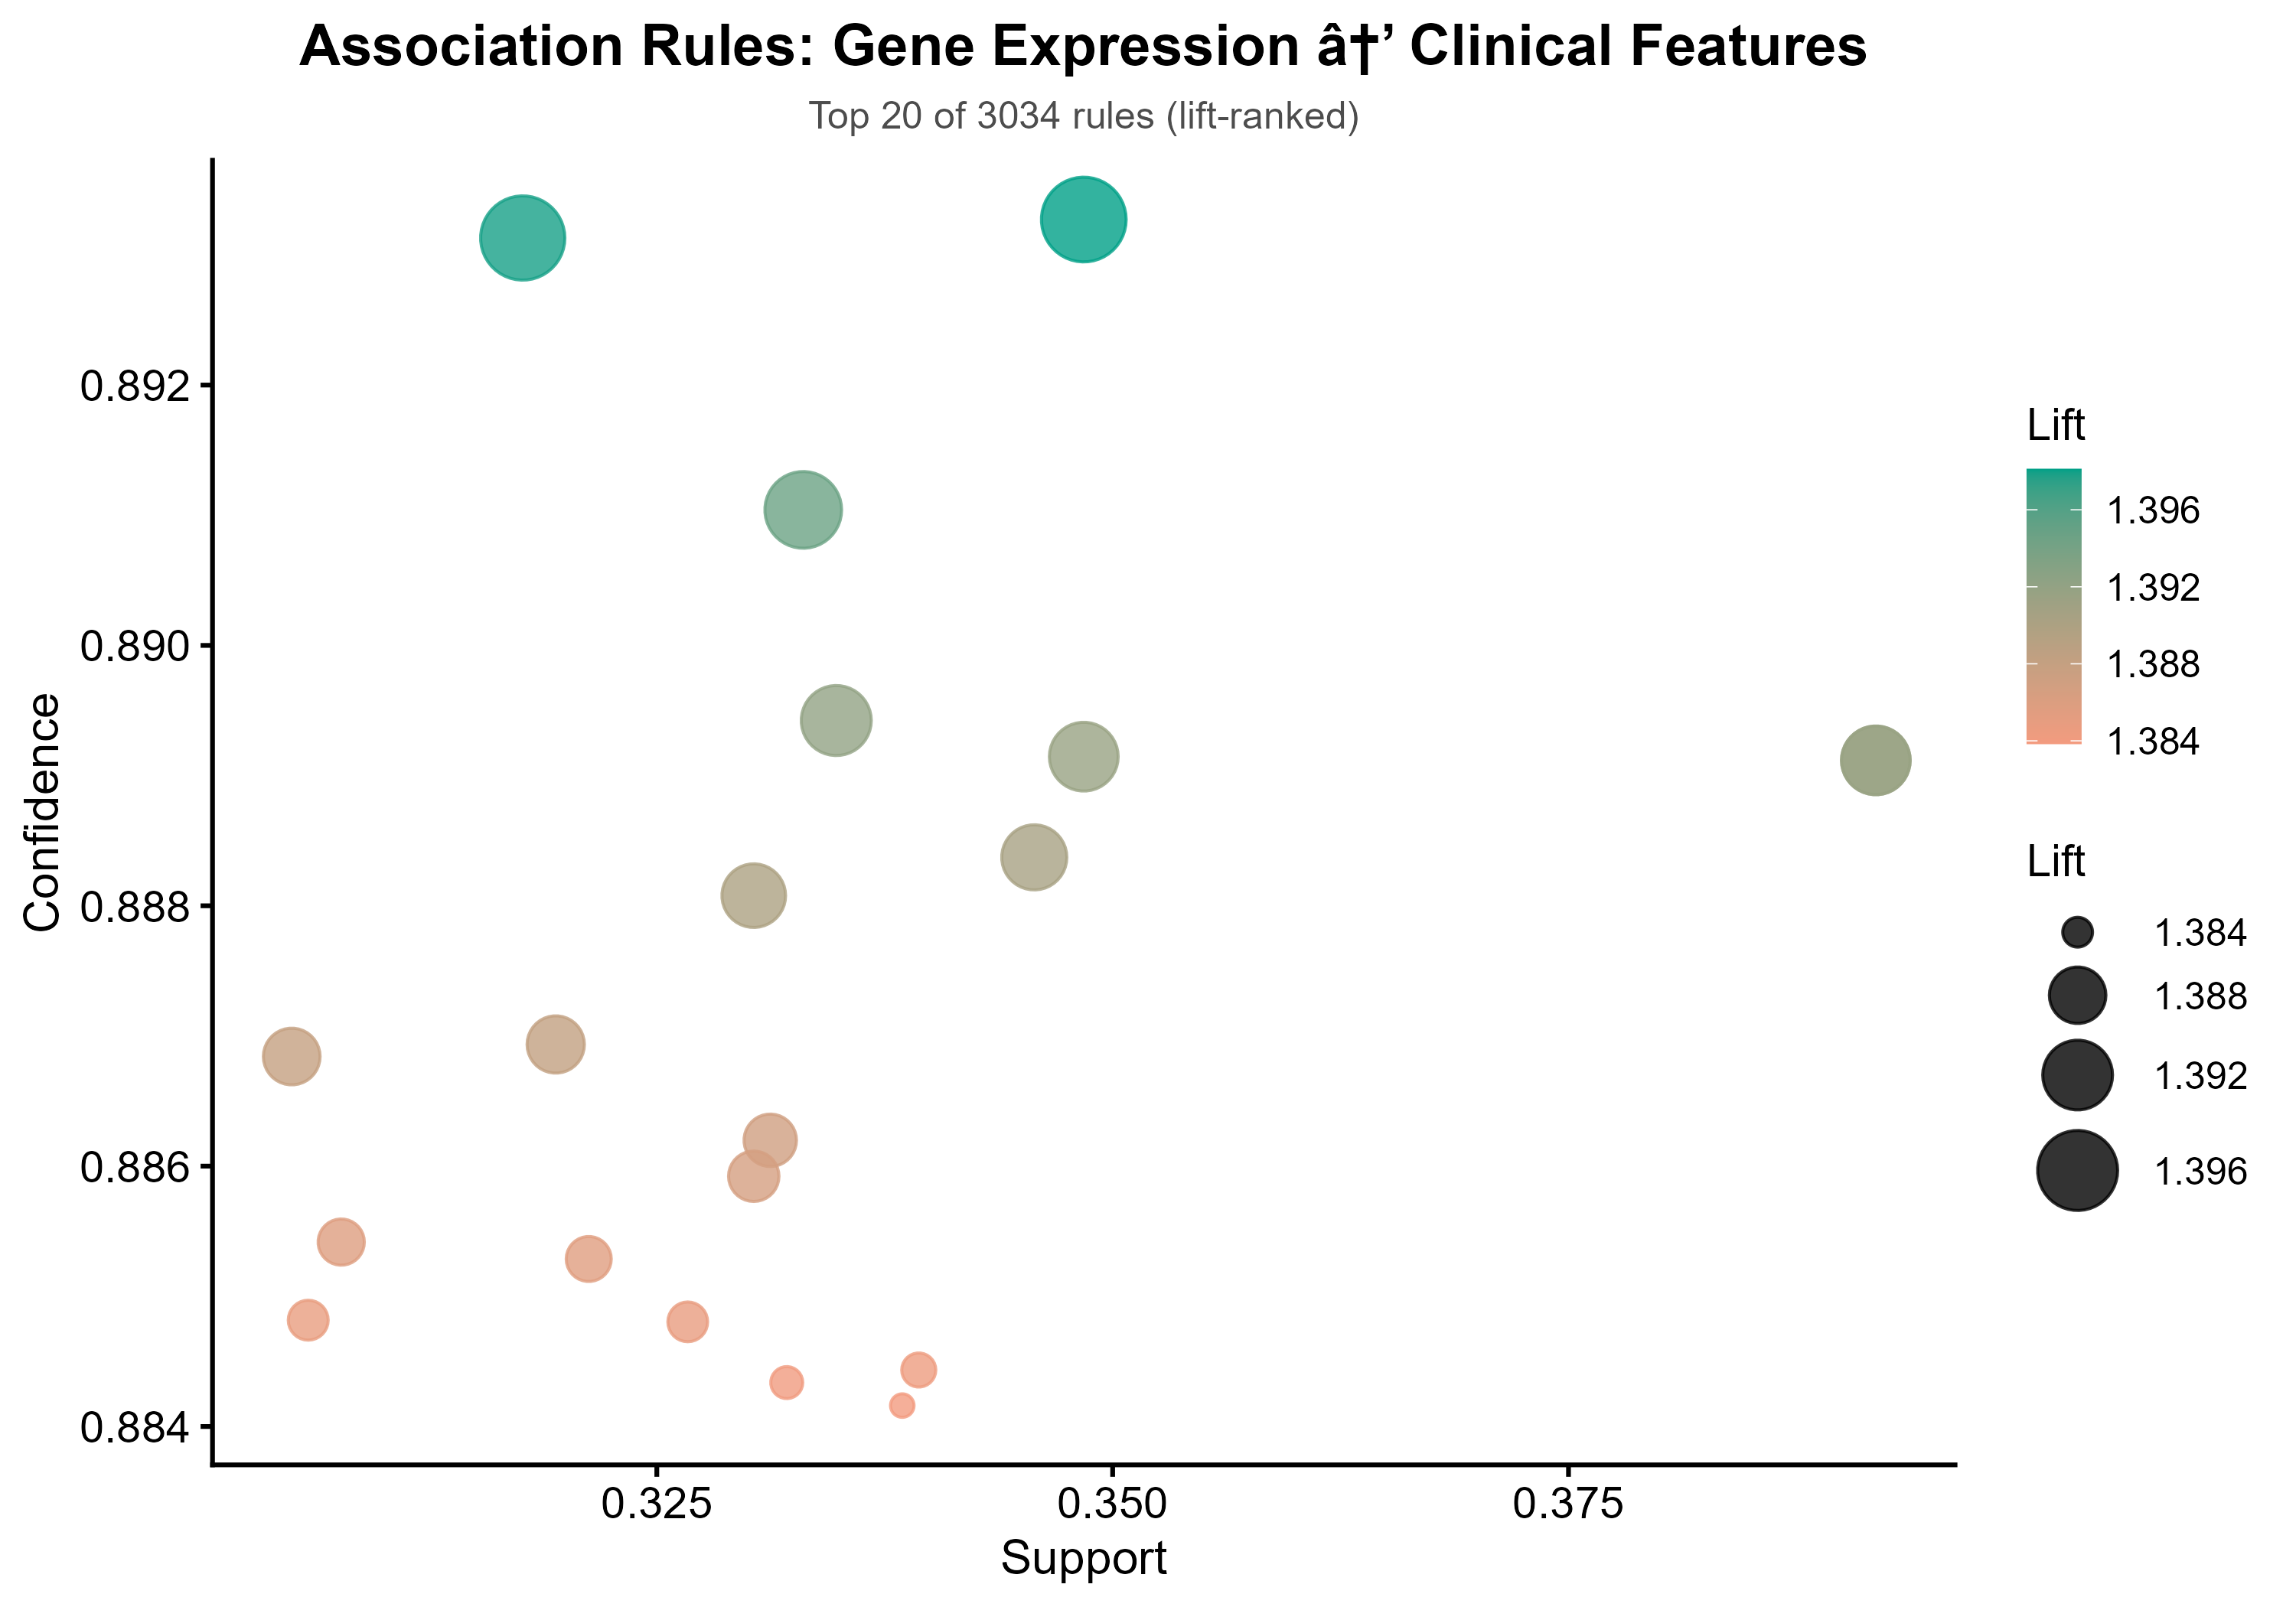
\includegraphics[width=0.8\textwidth]{fig15_association_rules.png}
\caption{关联规则散点图（Support $\times$ Confidence, Lift着色）}
\label{fig:rules}
\end{figure}

\begin{figure}[H]
\centering
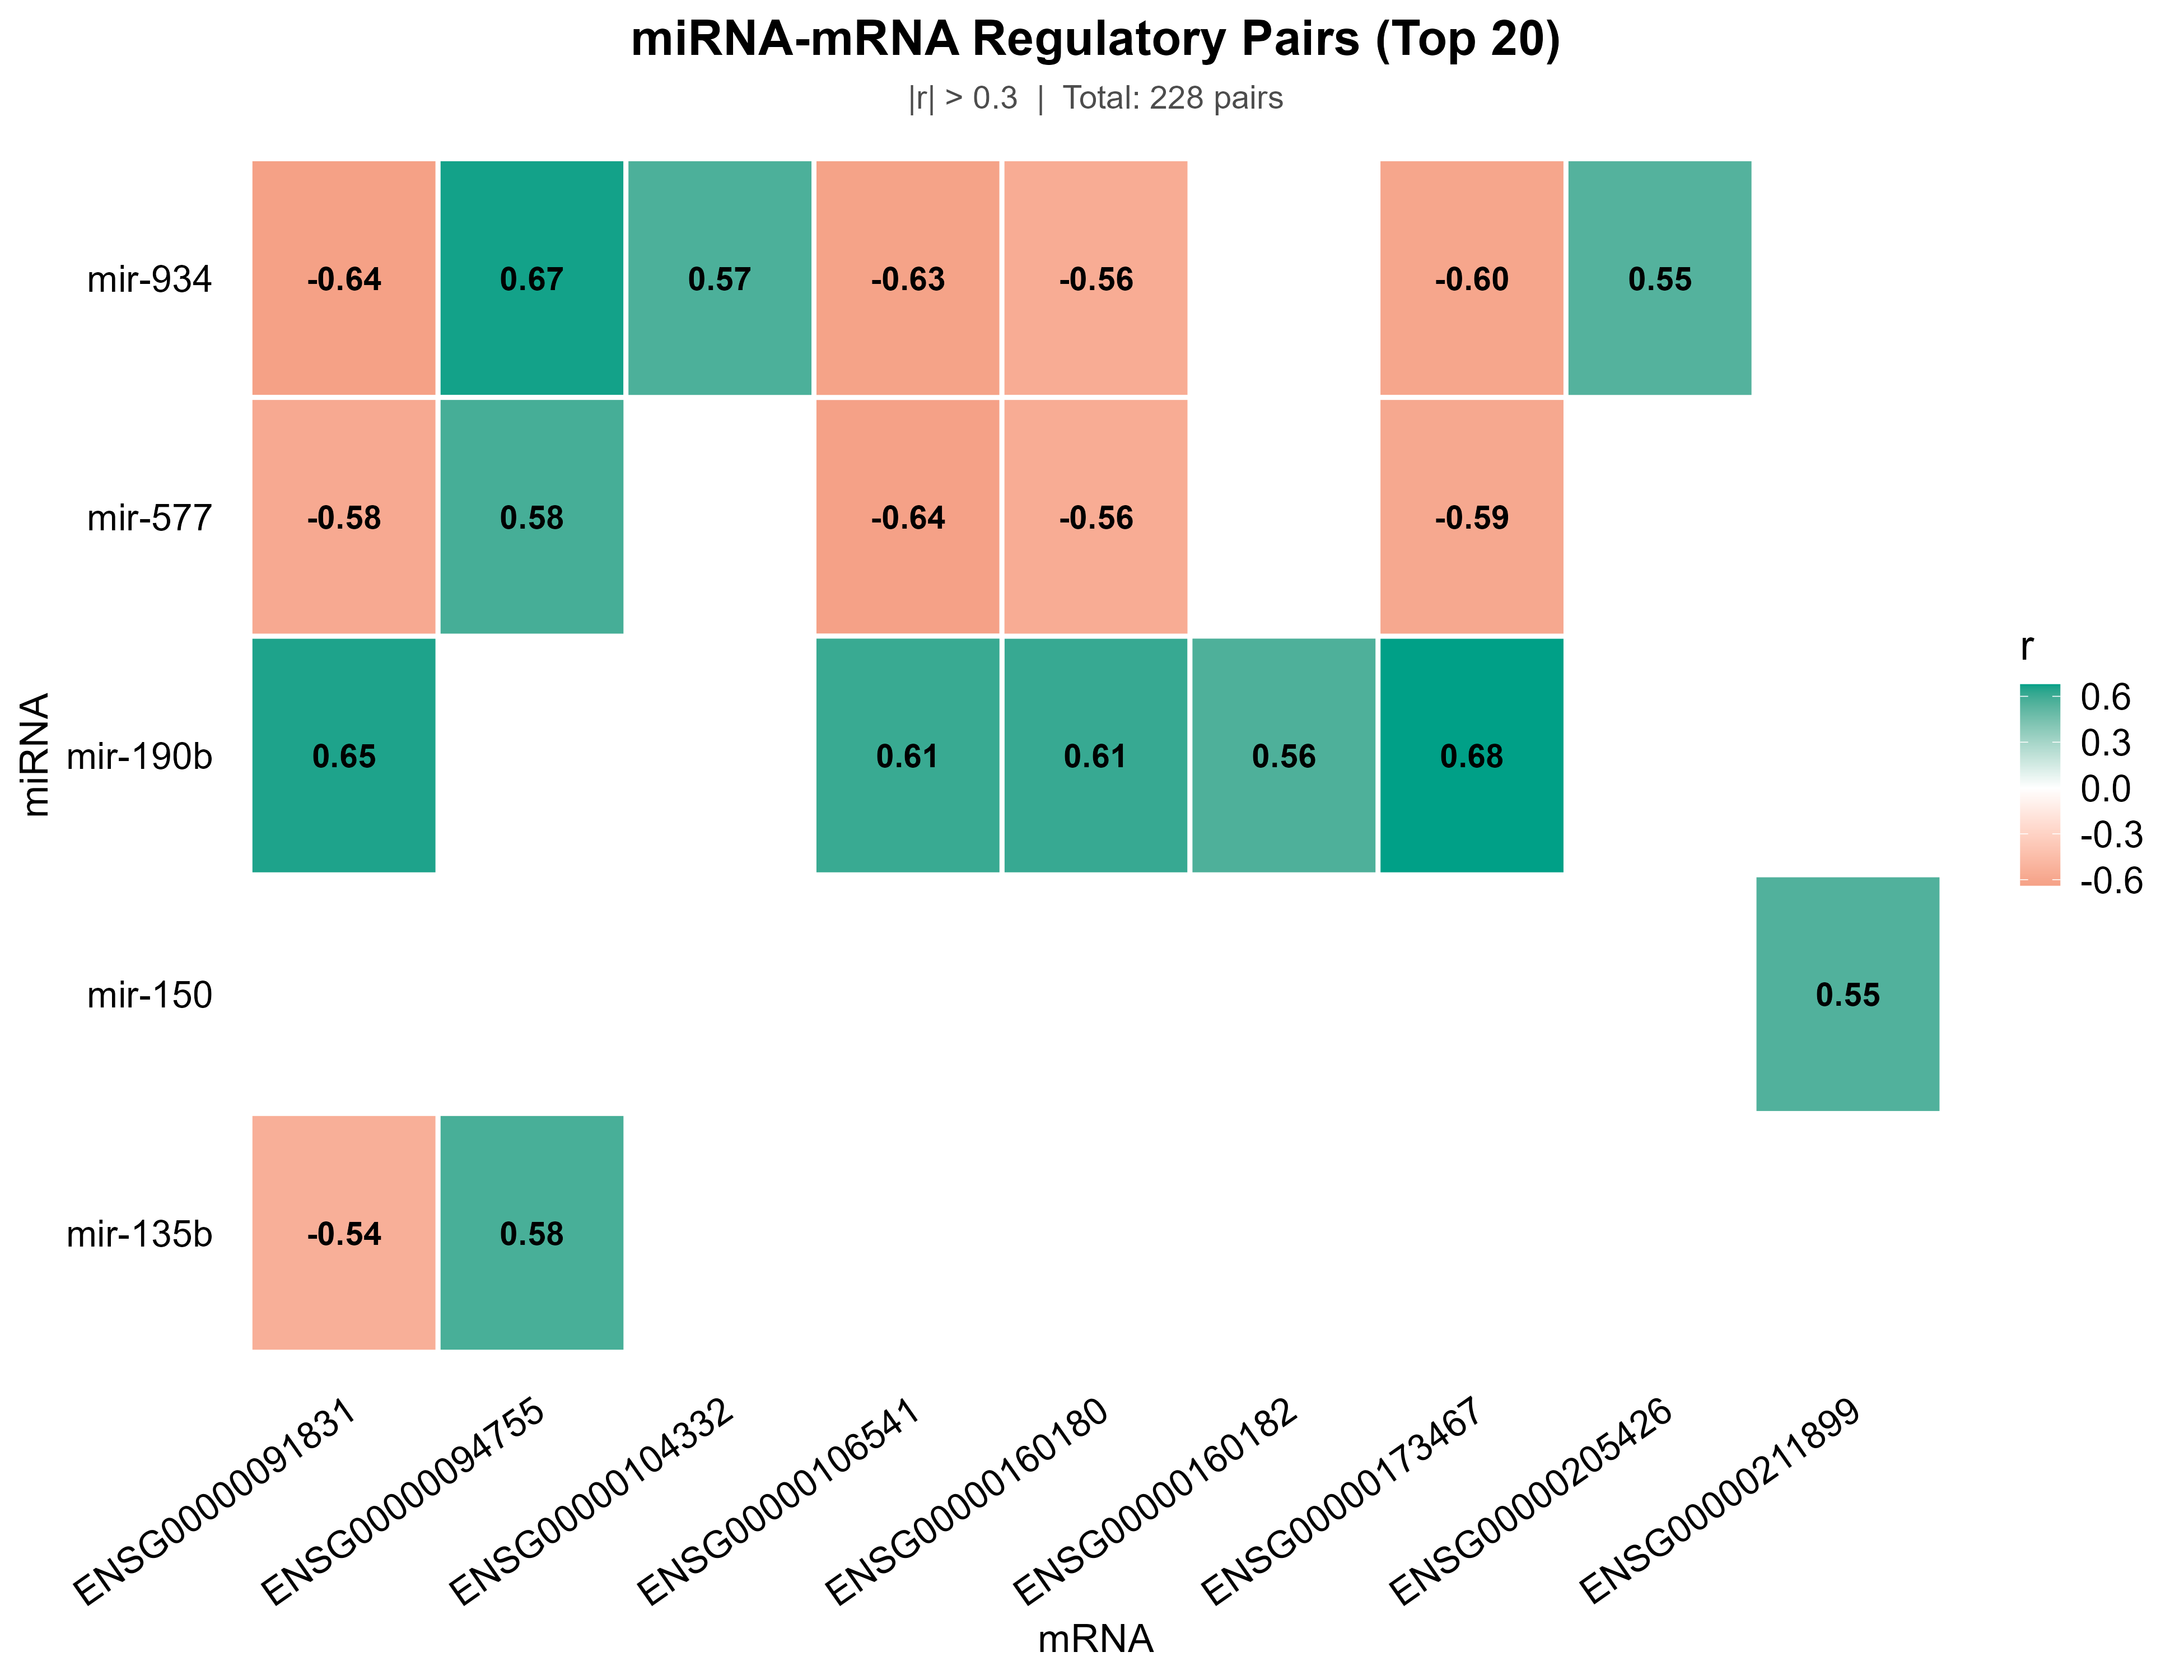
\includegraphics[width=0.85\textwidth]{fig10_mirna_mrna_corr.png}
\caption{miRNA-mRNA调控相关性热图（Top 20, $|r|>0.4$）}
\label{fig:mirna}
\end{figure}

% ==================== 4 可视化分析 ====================
\section{可视化分析}

本研究所有图表遵循统一规范：PNG格式，300 DPI分辨率，NPG（Nature Publishing Group）学术色板，英文标注。

图\ref{fig:heatmap}为Top 25 DEGs的聚类热图，以Z-score标准化展示肿瘤与正常的表达模式差异。两个主要样本聚类分支清晰分离，仅极少数样本交叉。图\ref{fig:enrich_comp}比较了上调与下调基因在六个来源数据库中的富集条目分布。图\ref{fig:summary}为六面板综合分析汇总图。

\begin{figure}[H]
\centering
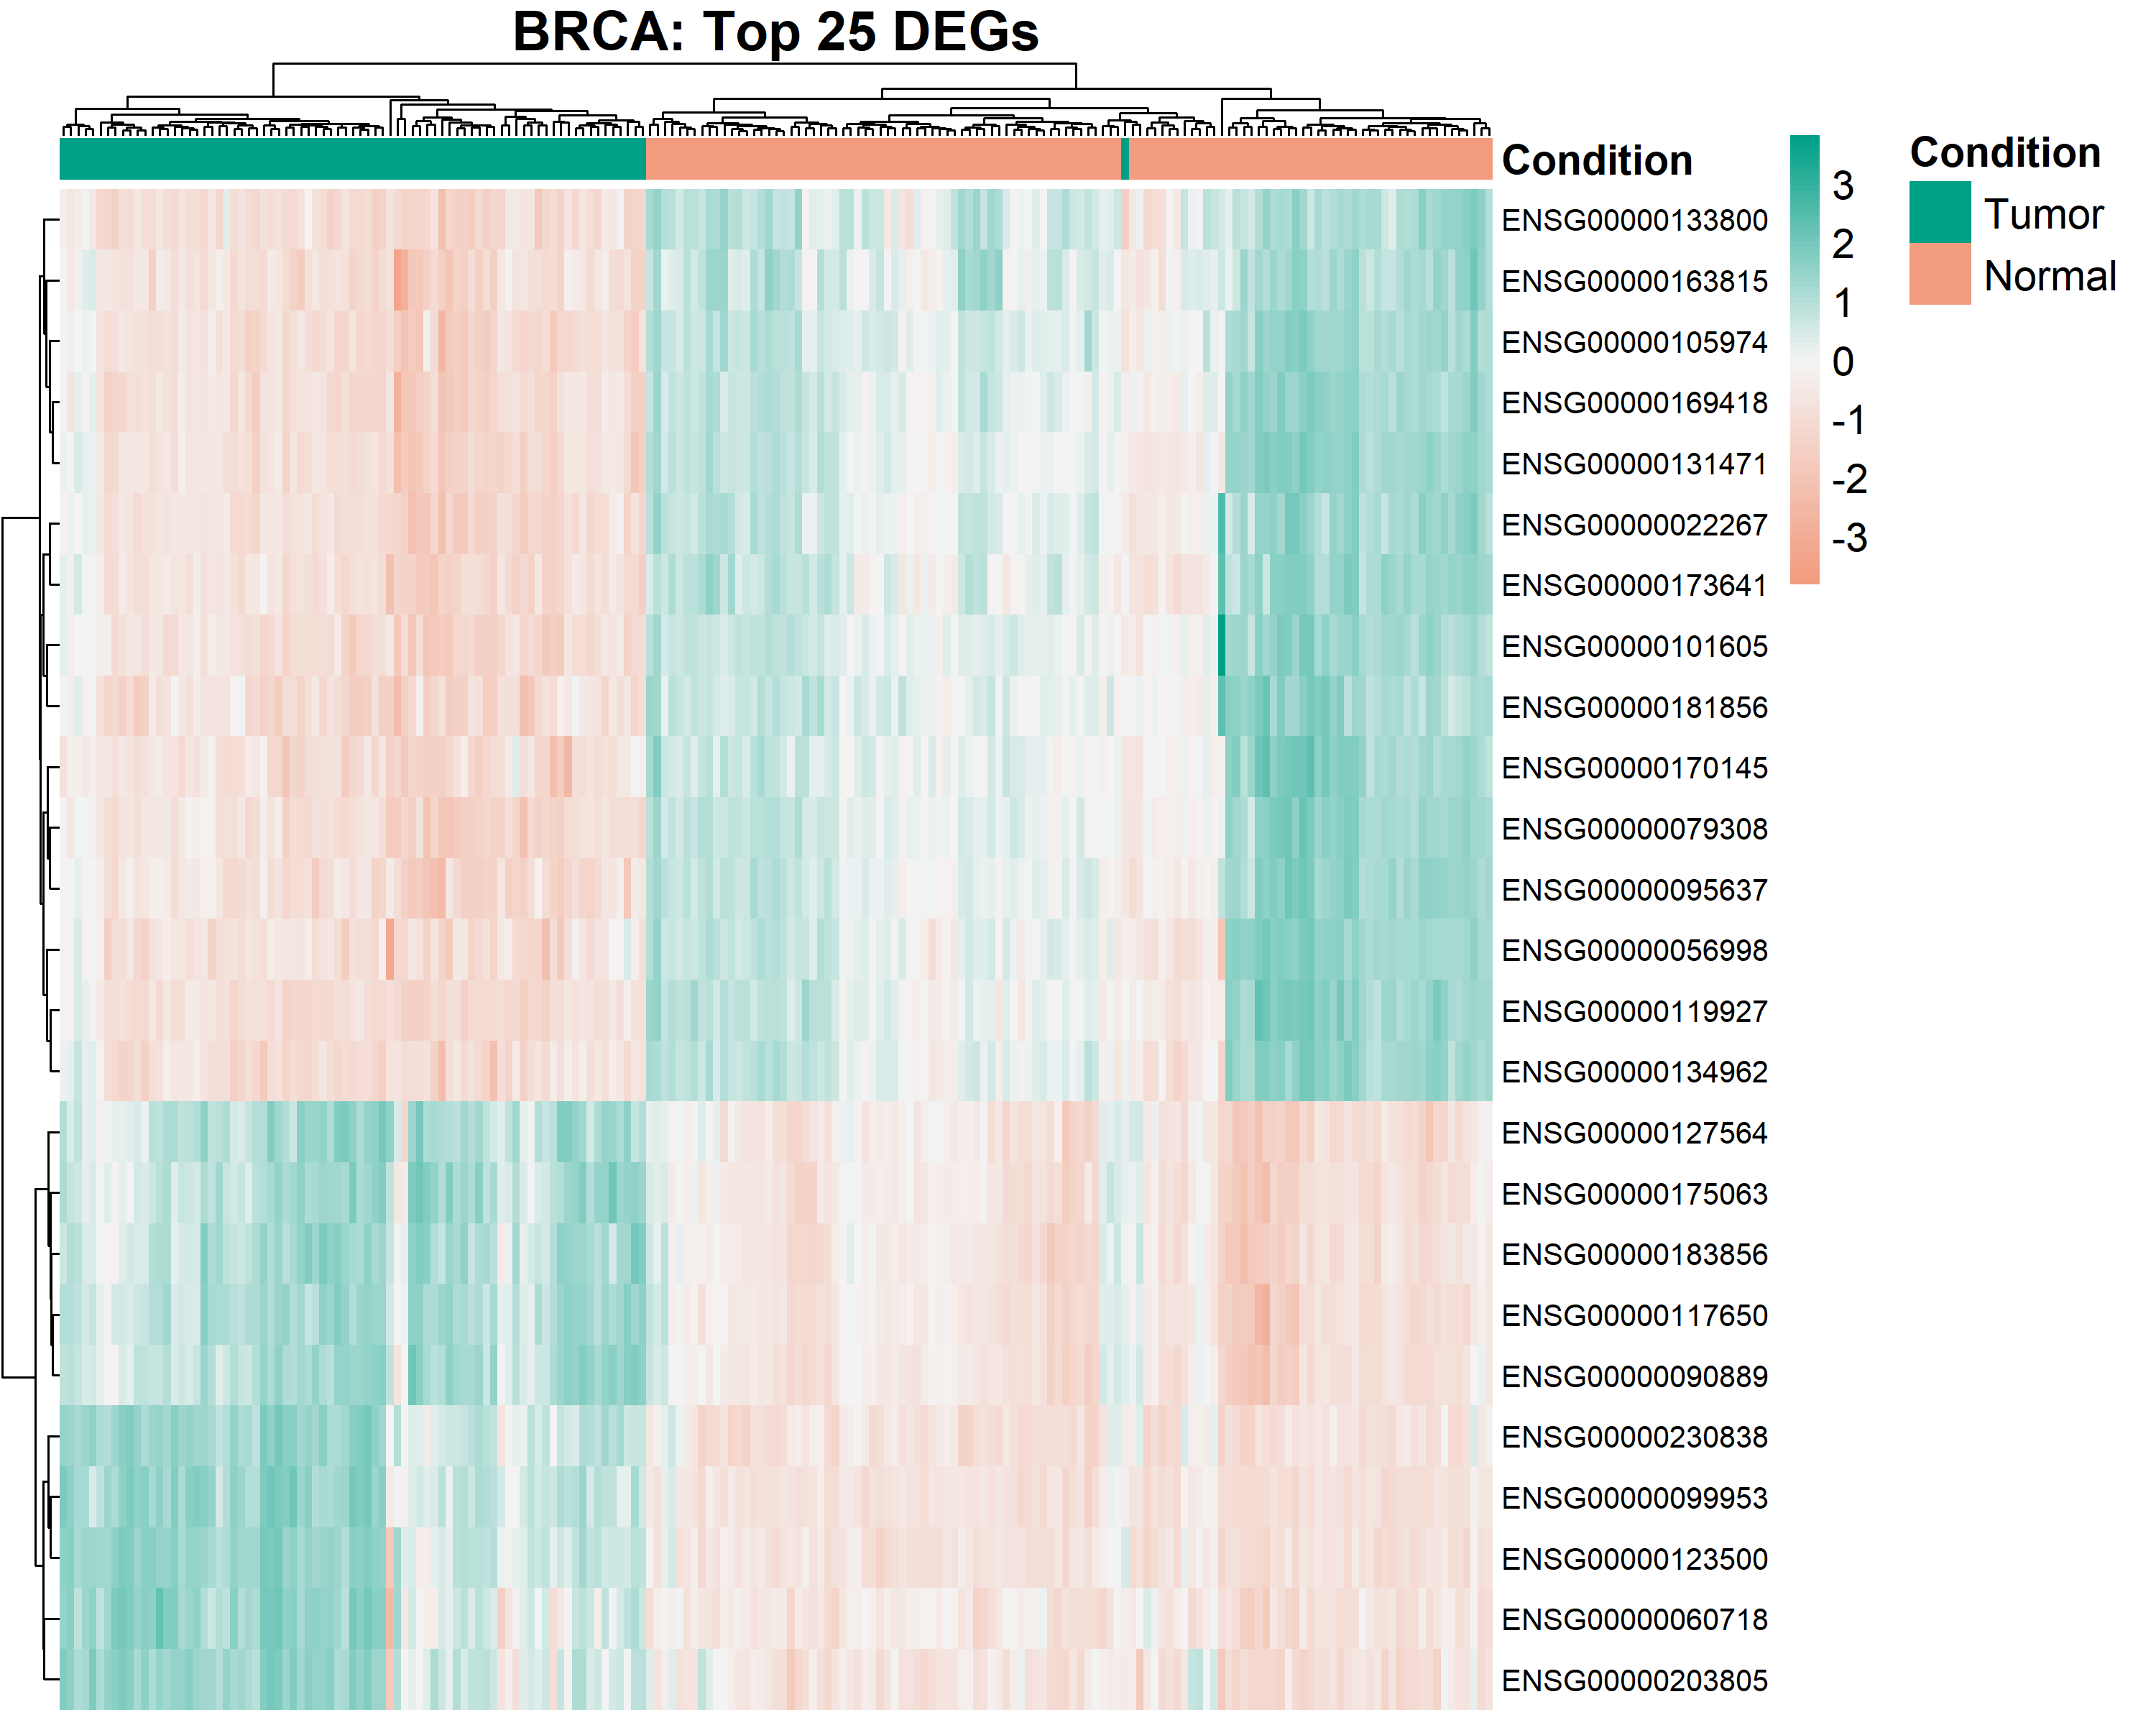
\includegraphics[width=0.85\textwidth]{fig5_deg_heatmap.png}
\caption{Top 25 DEGs表达热图（Tumor vs Normal, Z-score标准化）}
\label{fig:heatmap}
\end{figure}

\begin{figure}[H]
\centering
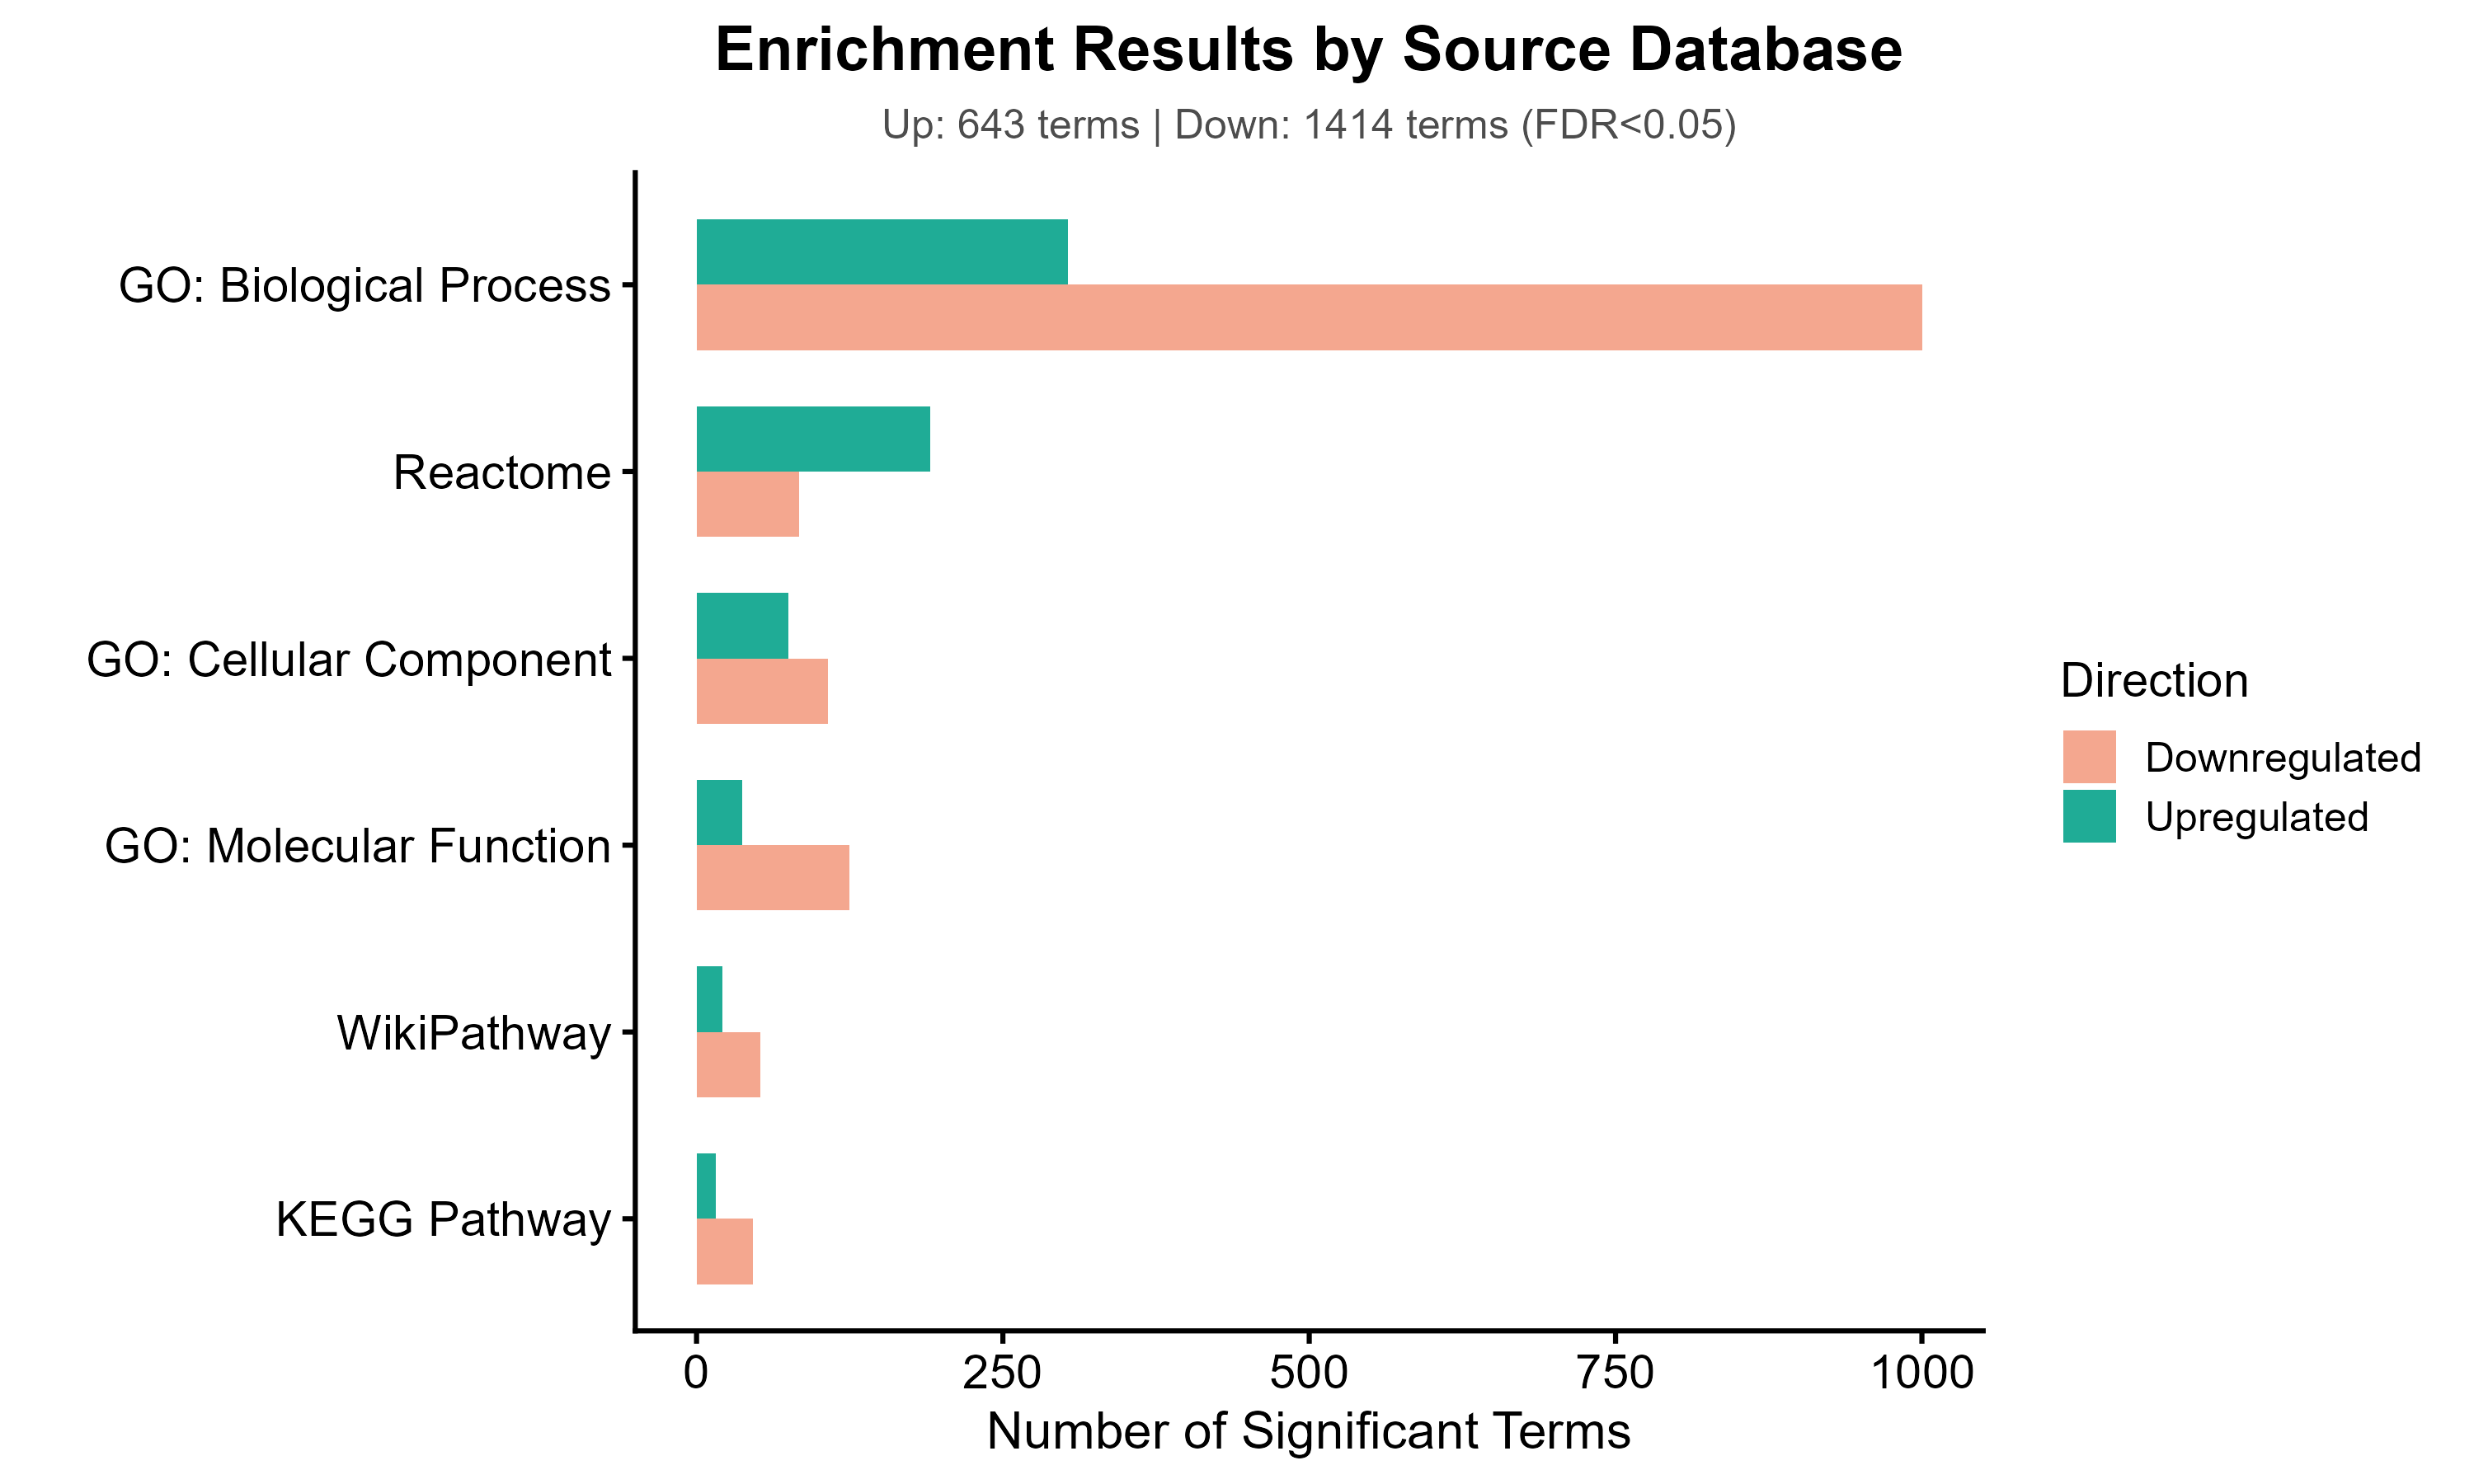
\includegraphics[width=0.8\textwidth]{fig14_enrichment_comparison.png}
\caption{富集来源数据库对比（上调 vs 下调）}
\label{fig:enrich_comp}
\end{figure}

\begin{figure}[H]
\centering
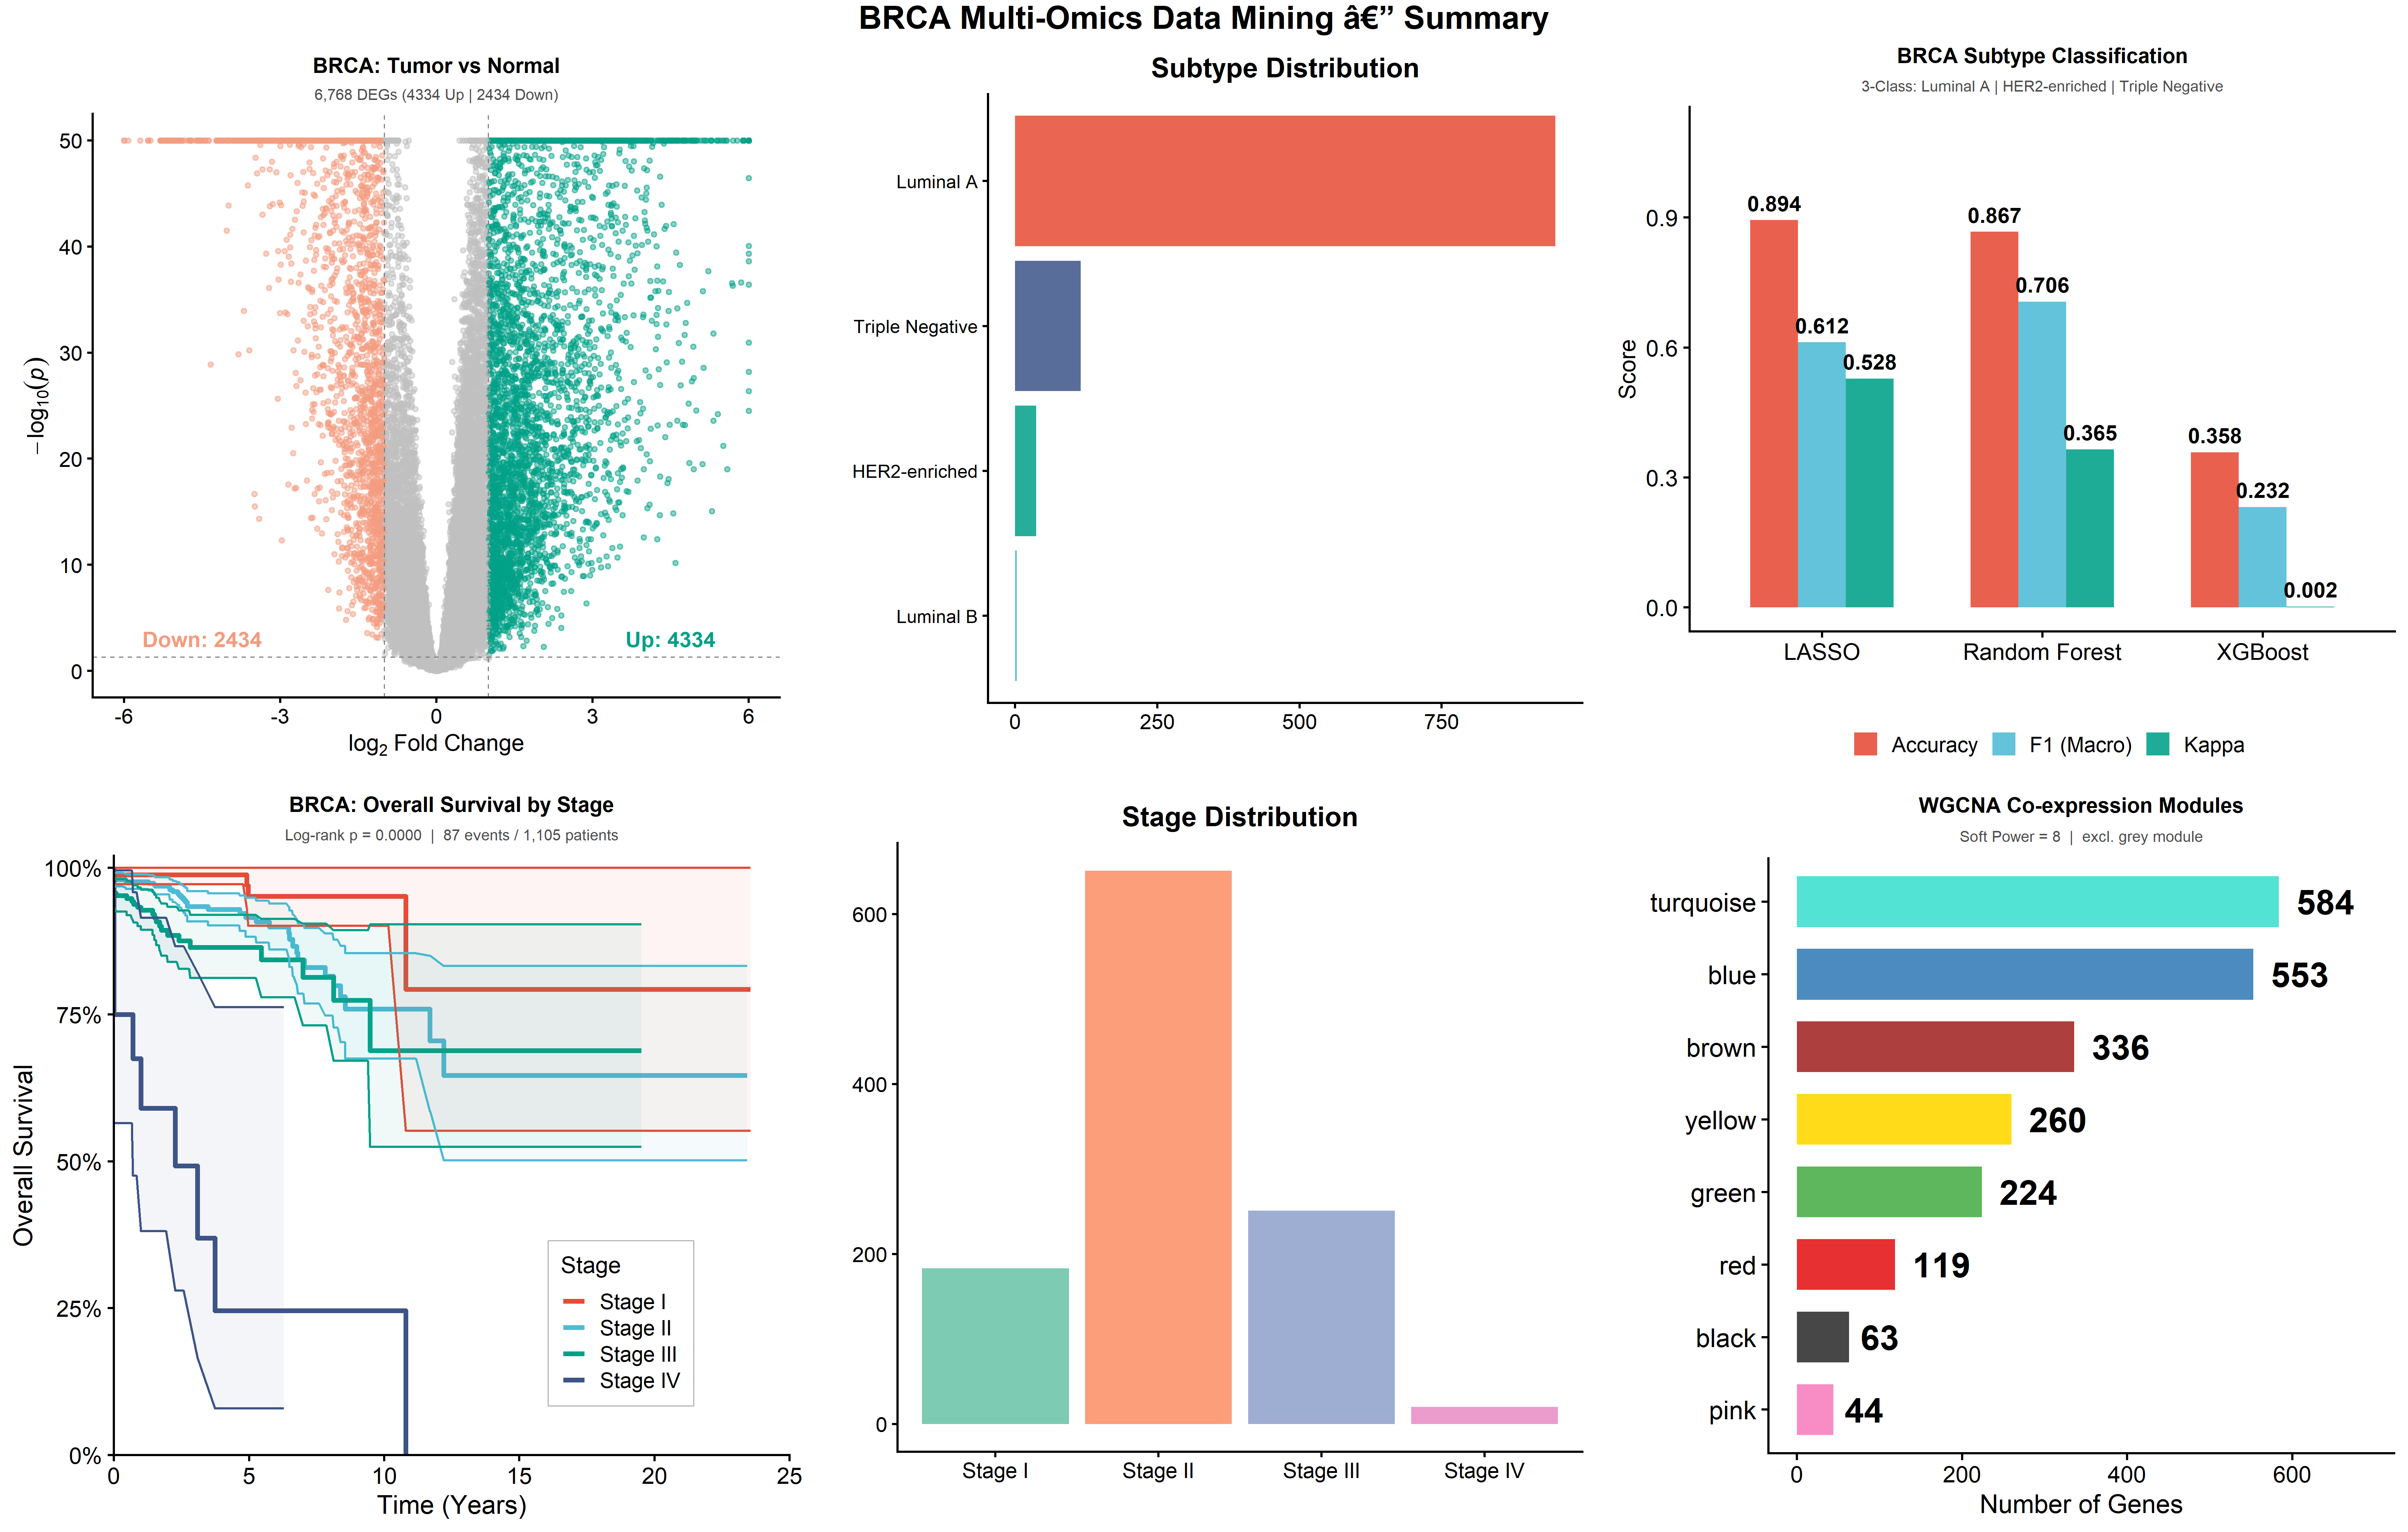
\includegraphics[width=\textwidth]{fig11_summary.png}
\caption{综合分析六面板汇总图}
\label{fig:summary}
\end{figure}

% ==================== 5 结论与展望 ====================
\section{结论与展望}

本研究以TCGA-BRCA乳腺癌队列为数据基础，整合mRNA、miRNA和体细胞突变三个组学层次，构建了覆盖差异表达分析、功能富集、分子亚型分类、聚类分析、WGCNA共表达网络、生存分析、突变分析及关联规则挖掘等九个分析模块的完整数据挖掘流程。

主要发现包括：（1）DESeq2鉴定6,768个显著差异基因，功能富集揭示上调基因集中于细胞周期通路（$p=1.5\times10^{-21}$），下调基因集中于ECM组织通路；（2）LASSO以89.4\%准确率仅用35个基因实现分子亚型三分类，验证了亚型间转录组差异的稀疏性；（3）PCA和K-means一致表明ER状态是BRCA转录组结构的最强驱动因素；（4）WGCNA识别9个共表达模块，Blue模块枢纽基因MM达0.959；（5）多变量Cox证实病理分期为BRCA预后最强预测因子（C-index=0.771, Stage IV HR=8.74）；（6）PIK3CA（37.3\%）和TP53（35.2\%）确认为BRCA最高频驱动突变，两者呈现互斥趋势；（7）关联规则挖掘识别了基因表达与临床特征之间的系统性关联模式。

本研究存在以下局限性：DNA甲基化数据因数据量过大（11.7 GB）未纳入分析；生存分析事件率较低（7.9\%）限制了多变量预后模型的统计功效；miRNA-mRNA调控关系基于统计相关而非因果验证。未来研究方向包括：采用降采样策略纳入DNA甲基化数据实现四组学整合；利用独立验证队列（METABRIC、SCAN-B）进行外部验证；对WGCNA Blue模块枢纽基因进行功能实验验证；以及探索深度学习方法在多组学数据融合中的应用前景。

% ==================== 参考文献 ====================
\printbibliography

\end{document}
